\documentclass[11pt,a4paper]{article}

% ---------------------------------------------------------------- pacotes
\usepackage[T1]{fontenc}
\usepackage[utf8]{inputenc}
\usepackage[english,brazilian]{babel}
\usepackage{lmodern}
\usepackage{microtype}
\usepackage[margin=2.4cm]{geometry}
\usepackage{amsmath,amssymb,amsthm,mathtools}
\usepackage{graphicx}
\usepackage{booktabs,tabularx,multirow}
\usepackage{siunitx}
\usepackage{xcolor}
\usepackage{caption,subcaption}
\usepackage{enumitem}
\usepackage{algorithm}
\usepackage{algpseudocode}
\usepackage[backend=biber,style=numeric-comp,sorting=nyt,maxbibnames=6,giveninits=true]{biblatex}
\usepackage[hidelinks]{hyperref}
\usepackage[capitalise,nameinlink,brazilian]{cleveref}

\addbibresource{refs.bib}
\emergencystretch=1.5em
\graphicspath{{../experiments/figures/}{../docs/img/}}
\sisetup{group-separator={\,},group-minimum-digits=4,output-decimal-marker={,}}
\floatname{algorithm}{Algoritmo}
\renewcommand{\algorithmicrequire}{\textbf{Entrada:}}
\renewcommand{\algorithmicensure}{\textbf{Saída:}}

\theoremstyle{plain}
\newtheorem{theorem}{Teorema}
\newtheorem{proposition}[theorem]{Proposição}
\newtheorem{lemma}[theorem]{Lema}
\newtheorem{corollary}[theorem]{Corolário}
\theoremstyle{definition}
\newtheorem{definition}[theorem]{Definição}
\newtheorem{example}[theorem]{Exemplo}
\theoremstyle{remark}
\newtheorem{remark}[theorem]{Observação}
\crefname{theorem}{Teorema}{Teoremas}
\crefname{proposition}{Proposição}{Proposições}
\crefname{definition}{Definição}{Definições}
\crefname{lemma}{Lema}{Lemas}

% marcadores de procedência dos resultados
\newcommand{\lit}{\textsuperscript{[L]}}  % resultado conhecido da literatura
\newcommand{\ver}{\textsuperscript{[V]}}  % verificado computacionalmente neste projeto
\newcommand{\proj}{\textsuperscript{[P]}} % contribuição/observação deste projeto

\newcommand{\Sym}{\operatorname{Sym}}
\newcommand{\sgn}{\operatorname{sgn}}
\newcommand{\Cay}{\operatorname{Cay}}
\newcommand{\cube}[1]{$#1\times#1\times#1$}
\newcommand{\mv}[1]{\texttt{#1}}

\makeatletter\newcommand{\inputtab}[1]{\@@input #1 }\makeatother
% Arquivo GERADO por experiments/analysis/analyze.py — não editar à mão.
\newcommand{\gclBfsTimeHTM}{\num{414}}
\newcommand{\gclBfsTimeQTM}{\num{331}}
\newcommand{\gclDiamHTM}{\num{11}}
\newcommand{\gclDiamQTM}{\num{14}}
\newcommand{\gclEfourMaxNodes}{\num{1000000}}
\newcommand{\gclEfourRUTwoDiamH}{\num{14}}
\newcommand{\gclEfourRUTwoDiamQ}{\num{17}}
\newcommand{\gclEfourRUtwoThreeDiam}{\num{25}}
\newcommand{\gclEfourSets}{\num{17}}
\newcommand{\gclEfourSqDiam}{\num{15}}
\newcommand{\gclEfourSqMean}{\num{10.13}}
\newcommand{\gclEoneFirstGap}{\num{5}}
\newcommand{\gclEoneGrowthBFS}{\num{5.05}}
\newcommand{\gclEoneGrowthBi}{\num{2.49}}
\newcommand{\gclEoneGrowthRatio}{\num{2.25}}
\newcommand{\gclEoneMaxL}{\num{20}}
\newcommand{\gclEoneRhoD}{\num{0.986}}
\newcommand{\gclEoneRhoL}{\num{0.827}}
\newcommand{\gclEoneSamples}{\num{30}}
\newcommand{\gclEoneSatMean}{\num{8.74}}
\newcommand{\gclEthreeAllOptimal}{todas}
\newcommand{\gclEthreeLastD}{\num{11}}
\newcommand{\gclEthreeMaxExp}{\num{33670}}
\newcommand{\gclEthreeMaxOverOri}{\num{14.5}}
\newcommand{\gclEthreeMaxOverPerm}{\num{5.5}}
\newcommand{\gclEthreeMisFailFrom}{\num{11}}
\newcommand{\gclEthreeMisMax}{\num{2}}
\newcommand{\gclEthreeNodeLimit}{\num{3000000}}
\newcommand{\gclEthreeSamples}{\num{15}}
\newcommand{\gclEthreeShowCols}{4}
\newcommand{\gclEthreeZeroFailFrom}{\num{8}}
\newcommand{\gclEthreebCount}{\num{90}}
\newcommand{\gclEthreebDstarEqL}{sim}
\newcommand{\gclEthreebDstarEqLCount}{\num{90}}
\newcommand{\gclEthreebLmax}{\num{12}}
\newcommand{\gclEthreebPdbExpLast}{\num{1120950}}
\newcommand{\gclEthreebPdbTimeLast}{\num{4.5}}
\newcommand{\gclEthreebSamples}{\num{10}}
\newcommand{\gclEthreebTPExcessMax}{\num{8}}
\newcommand{\gclEthreebTPOptimalPct}{\num{97}}
\newcommand{\gclEtwoAllOptimal}{todas}
\newcommand{\gclEtwoAstarExp}{\num{19562}}
\newcommand{\gclEtwoAstarPeak}{\num{100822}}
\newcommand{\gclEtwoAstarTime}{\num{48.4}}
\newcommand{\gclEtwoBFSBiExp}{\num{14456}}
\newcommand{\gclEtwoBFSBiPeak}{\num{74584}}
\newcommand{\gclEtwoBFSBiTime}{\num{15.8}}
\newcommand{\gclEtwoBFSExp}{\num{3191043}}
\newcommand{\gclEtwoBFSPeak}{\num{3672938}}
\newcommand{\gclEtwoBFSTime}{\num{1222.1}}
\newcommand{\gclEtwoDmax}{\num{11}}
\newcommand{\gclEtwoIDAstarExp}{\num{36544}}
\newcommand{\gclEtwoIDAstarPeak}{\num{11}}
\newcommand{\gclEtwoIDAstarTime}{\num{11.7}}
\newcommand{\gclEtwoRuns}{\num{880}}
\newcommand{\gclEtwoSamples}{\num{20}}
\newcommand{\gclEzeroAllMatch}{todas}
\newcommand{\gclGhtmSpheres}{\num{1}; \num{18}; \num{243}; \num{3240}; \num{43239}; \num{574908}}
\newcommand{\gclGqtmSpheres}{\num{1}; \num{12}; \num{114}; \num{1068}; \num{10011}; \num{93840}; \num{878880}}
\newcommand{\gclMeanDistHTM}{\num{8.756}}
\newcommand{\gclMeanDistQTM}{\num{10.666}}
\newcommand{\gclResultsCommit}{8585968}
\newcommand{\gclResultsDate}{2026-11-09}
\newcommand{\gclResultsEnv}{node v22.23.4; Linux 6.18.44-fc-v310 x64; CPU Intel(R) Xeon(R) Processor @ 2.10GHz $\times$4; RAM 15.7 GiB}
\newcommand{\gclResultsTotalMin}{\num{10.7}}
\newcommand{\gclSchreierGTime}{\num{7.7}}
\newcommand{\gclTPFirstLe}{\num{2}}
\newcommand{\gclTPFirstMax}{\num{26}}
\newcommand{\gclTPFirstMean}{\num{23.15}}
\newcommand{\gclTPFirstMin}{\num{19}}
\newcommand{\gclTPFirstTimeMax}{\num{62}}
\newcommand{\gclTPFirstTimeMed}{\num{4.4}}
\newcommand{\gclTPTargetLe}{\num{82}}
\newcommand{\gclTPTargetMax}{\num{21}}
\newcommand{\gclTPTargetMean}{\num{20.04}}
\newcommand{\gclTPTargetMin}{\num{19}}
\newcommand{\gclTPTargetTimeMax}{\num{1012}}
\newcommand{\gclTPTargetTimeMed}{\num{115.2}}
\newcommand{\gclTPUniformN}{\num{100}}
\newcommand{\gclTwoPhaseTables}{\num{1310}}


\title{\textbf{GraphCube Lab}: fundamentos matemáticos, representações em grafos\\ e algoritmos computacionais para o cubo mágico\\[0.4em]
\large\textit{GraphCube Lab: Mathematical Foundations, Graph Representations and Computational Algorithms for the Rubik's Cube}}
\author{Augusto Farias\thanks{Projeto de portfólio em Matemática Aplicada e Computacional. Código, dados e este texto: repositório \texttt{graphcube-lab}. Contato: \texttt{claude.augusto.farias@gmail.com}.}}
\date{Novembro de 2026 --- versão do software \texttt{0.1.0}}

\begin{document}
\maketitle

\begin{abstract}
\noindent
Este trabalho apresenta o GraphCube Lab, uma plataforma aberta, interativa e reprodutível para o estudo do cubo mágico com ferramentas de teoria dos grupos, teoria dos grafos e busca heurística. Partindo de uma análise do projeto GraphCube, mostramos que sua representação visual é um diagrama de incidência entre posições de adesivos e camadas --- e não um grafo de estados nem um grafo de Cayley --- e distinguimos formalmente essas três estruturas. O núcleo matemático deriva todas as permutações de uma única descrição geométrica dos adesivos, adota uma convenção de composição explícita e é validado contra resultados conhecidos: o algoritmo de Schreier--Sims reproduz $|G| = \num{43252003274489856000}$ e as ordens de seis subgrupos, e a busca em largura completa do \cube{2} reproduz a distribuição de distâncias publicada nas métricas HTM e QTM. Implementamos BFS, BFS bidirecional, A$^*$ e IDA$^*$ sobre grafos implícitos, heurísticas admissíveis e consistentes obtidas por projeções (\textit{pattern databases}) e o método de duas fases de Kociemba, sempre distinguindo algoritmos que garantem caminhos mínimos dos que produzem apenas soluções válidas. Experimentos com sementes registradas mostram, entre outros resultados, que o comprimento do embaralhamento é um mau substituto para a distância real (que satura em torno da média uniforme \gclMeanDistHTM{}), que a busca bidirecional reduz o crescimento por camada de \gclEoneGrowthBFS{} para \gclEoneGrowthBi{}, que a combinação de duas \textit{pattern databases} reduz os nós expandidos por IDA$^*$ em \gclEthreeMaxOverPerm{}$\times$ em relação à melhor delas isolada, e quantificam a estrutura de grafos de Cayley de \gclEfourSets{} conjuntos de geradores. Todas as visualizações parciais são rotuladas como tais e as animações de busca reproduzem o registro real de execução.

\medskip\noindent\textbf{Palavras-chave:} cubo mágico; teoria dos grupos; grafos de Cayley; algoritmos de busca; heurísticas admissíveis; visualização científica; reprodutibilidade.
\end{abstract}

\begin{otherlanguage}{english}
\begin{abstract}
\noindent
We present GraphCube Lab, an open, interactive and reproducible platform for studying the Rubik's cube through group theory, graph theory and heuristic search. Starting from an analysis of the GraphCube project, we show that its visual representation is a sticker--layer incidence diagram --- neither a state graph nor a Cayley graph --- and formally distinguish these three structures. The mathematical core derives every permutation from a single geometric description of the stickers, uses an explicit composition convention and is validated against known results: the Schreier--Sims algorithm reproduces $|G| = \num{43252003274489856000}$ and the orders of six subgroups, and an exhaustive breadth-first search of the $2\times2\times2$ cube reproduces its published distance distribution in both HTM and QTM. We implement BFS, bidirectional BFS, A$^*$ and IDA$^*$ over implicit graphs, admissible and consistent heuristics obtained from projections (pattern databases) and Kociemba's two-phase method, always separating algorithms that guarantee shortest paths from those that only return valid solutions. Seeded experiments show, among other results, that scramble length is a poor proxy for the true distance, that bidirectional search lowers the per-layer growth rate from \gclEoneGrowthBFS{} to \gclEoneGrowthBi{}, that combining two pattern databases reduces IDA$^*$ expansions by a factor of \gclEthreeMaxOverPerm{} over the best single one, and quantify the structure of Cayley graphs for \gclEfourSets{} generating sets. Partial visualisations are labelled as such and search animations replay the actual execution log.

\medskip\noindent\textbf{Keywords:} Rubik's cube; group theory; Cayley graphs; search algorithms; admissible heuristics; scientific visualisation; reproducibility.
\end{abstract}
\end{otherlanguage}

\section{Introdução}\label{sec:intro}

O cubo mágico é um dos exemplos mais conhecidos de \emph{quebra-cabeça de permutação}: seus estados são permutações de peças, seus movimentos geram um grupo finito e resolvê-lo equivale a encontrar uma palavra nos geradores que represente o inverso do estado atual. Essa formulação faz do cubo um laboratório natural para três áreas da Matemática Aplicada e Computacional: a \emph{teoria dos grupos}, que descreve quais estados são alcançáveis e como os movimentos se combinam~\cite{joyner2008,singmaster1981}; a \emph{teoria dos grafos}, que transforma o problema de resolução num problema de caminho mínimo num grafo de Cayley gigantesco~\cite{godsil2001,rokicki2014}; e a \emph{busca heurística}, que fornece algoritmos capazes de encontrar caminhos nesses grafos sem enumerá-los~\cite{hart1968,korf1985,korf1997}.

\paragraph{Motivação.} O projeto GraphCube~\cite{laguna2024} propôs uma visualização interativa elegante, em que famílias de círculos concêntricos representam as camadas do cubo e girar uma camada corresponde a deslizar pontos coloridos ao longo de um círculo. A proposta é visualmente atraente, mas não acompanha um modelo matemático explícito: não há representação de estados independente da tela, nem noção de grupo, distância ou algoritmo. Este trabalho parte dessa visualização para construir uma plataforma em que cada elemento gráfico tenha uma interpretação matemática precisa e verificável.

\paragraph{Trabalhos relacionados.} A estrutura de grupo do cubo é tratada em textos clássicos~\cite{singmaster1981,frey1982,joyner2008}. O diâmetro do grafo de Cayley do \cube{3} na métrica de meia-volta (HTM) foi determinado como 20 por Rokicki et al.~\cite{rokicki2014}, após uma série de cotas superiores como as 26 jogadas de Kunkle e Cooperman~\cite{kunkle2007}. Korf~\cite{korf1997} obteve as primeiras soluções ótimas para estados aleatórios combinando IDA$^*$~\cite{korf1985} com \textit{pattern databases}~\cite{culberson1998}, ideia depois estendida a heurísticas aditivas~\cite{felner2004}. O algoritmo de duas fases de Kociemba~\cite{kociemba1992,kociembaweb} encontra rapidamente soluções curtas, mas não necessariamente ótimas. Demaine et al.~\cite{demaine2011} estudaram a complexidade assintótica do cubo $n\times n\times n$, e abordagens recentes combinam aprendizado por reforço e busca~\cite{agostinelli2019}. Para o cálculo de ordens de grupos de permutação, o algoritmo de Schreier--Sims~\cite{sims1970,seress2003,holt2005} é a ferramenta padrão.

\paragraph{Objetivos e contribuições.} O objetivo não é produzir um resultado científico inédito sobre o cubo --- os resultados centrais são conhecidos --- mas construir uma ferramenta \emph{matematicamente rigorosa, reprodutível e didática} e documentar honestamente o que ela mostra. As contribuições deste trabalho são:
\begin{enumerate}[nosep,label=(\roman*)]
  \item uma análise do GraphCube que identifica precisamente o objeto que ele desenha (\cref{sec:graphcube}) e uma distinção formal entre grafo estrutural, grafo de estados e grafos de Cayley (\cref{sec:tres-grafos});
  \item um núcleo matemático em que todas as permutações derivam de uma descrição geométrica única, validado contra resultados da literatura (\cref{sec:modelagem,sec:res-validacao});
  \item a construção exata do diagrama de círculos do GraphCube como diagrama de incidência, generalizada para $n=2,3$ (\cref{sec:estrutural});
  \item implementações instrumentadas de BFS, BFS bidirecional, A$^*$, IDA$^*$ e do método de duas fases, com visualização que reproduz o registro real de cada execução (\cref{sec:desenvolvimento});
  \item quatro experimentos reprodutíveis sobre crescimento do espaço de busca, comparação de algoritmos, heurísticas e estrutura de grafos de Cayley (\cref{sec:metodologia,sec:resultados}).
\end{enumerate}

\paragraph{Procedência dos resultados.} Ao longo do texto, marcamos com \lit{} resultados conhecidos da literatura, com \ver{} resultados conhecidos que foram \emph{verificados computacionalmente} pelo nosso software e com \proj{} observações e medições produzidas especificamente neste projeto. Nenhuma afirmação de originalidade científica é feita além das contribuições de engenharia e de síntese acima.

\section{Fundamentação teórica}\label{sec:fundamentacao}

\subsection{Grupos de permutação}
Seja $\Omega$ um conjunto finito. O grupo simétrico $\Sym(\Omega)$ é o conjunto das bijeções de $\Omega$ com a composição. Neste trabalho adotamos explicitamente
\begin{equation}\label{eq:produto}
  (g\cdot h)(i) = g\bigl(h(i)\bigr), \qquad g,h\in\Sym(\Omega),\; i\in\Omega,
\end{equation}
isto é, $g\cdot h$ aplica primeiro $h$ e depois $g$ \emph{aos índices}. Toda permutação se decompõe, de modo único a menos da ordem, em ciclos disjuntos; a \emph{ordem} de $g$ (menor $k\ge1$ com $g^k=e$) é o mínimo múltiplo comum dos comprimentos desses ciclos, e o \emph{sinal} é $\sgn g = (-1)^{\sum_c (|c|-1)}$, um homomorfismo $\Sym(\Omega)\to\{\pm1\}$~\cite{joyner2008}. O \emph{comutador} de $a$ e $b$ é $[a,b]=a\,b\,a^{-1}b^{-1}$ e o \emph{conjugado} de $a$ por $b$ é $b\,a\,b^{-1}$; conjugados têm o mesmo tipo de ciclo\lit.

Dado $S\subseteq\Sym(\Omega)$, o subgrupo gerado $\langle S\rangle$ é o menor subgrupo que contém $S$. Uma \emph{base} $B=(\beta_1,\dots,\beta_k)$ e um \emph{conjunto gerador forte} definem a cadeia de estabilizadores $G=G^{(1)}\ge G^{(2)}\ge\cdots\ge G^{(k+1)}=1$, com $G^{(i+1)}=G^{(i)}_{\beta_i}$. Pelo teorema órbita-estabilizador, $|G|=\prod_i |\beta_i^{G^{(i)}}|$. O algoritmo de Schreier--Sims~\cite{sims1970,seress2003,holt2005} constrói essa cadeia a partir de geradores arbitrários, usando os geradores de Schreier $u_x s\, u_{xs}^{-1}$ e o teste de pertinência por peneiramento (\textit{sifting}).

\subsection{Grafos de Cayley}
\begin{definition}[Grafo de Cayley]
Sejam $H$ um grupo e $S\subseteq H\setminus\{e\}$ com $S=S^{-1}$. O grafo de Cayley $\Cay(H,S)$ tem vértices $H$ e arestas $\{h, h s\}$, $h\in H$, $s\in S$.
\end{definition}
\noindent $\Cay(H,S)$ é $|S|$-regular, conexo se e somente se $S$ gera $H$, e \emph{vértice-transitivo}: para cada $g\in H$, a multiplicação à esquerda $h\mapsto gh$ é um automorfismo~\cite{godsil2001}\lit. A distância $d(g,h)$ é o menor comprimento de uma palavra em $S$ que representa $g^{-1}h$; o \emph{diâmetro} é o maior $d(e,h)$; a \emph{esfera} de raio $r$ é $S(r)=\{h: d(e,h)=r\}$. Um ciclo que passa por $e$ corresponde a uma palavra $s_1\cdots s_k$ com produto $e$ que não se reduz livremente à palavra vazia --- uma \emph{relação} entre os geradores. A \emph{cintura} (\textit{girth}) é o comprimento do menor ciclo. Babai e Seress~\cite{babai1992} discutem cotas gerais para diâmetros de grafos de Cayley de grupos de permutação.

\subsection{Busca em grafos}
Dado um grafo com custos unitários, um estado inicial $s_0$ e um objetivo $t$:
\begin{itemize}[nosep]
\item a \textbf{busca em largura} (BFS) expande os vértices por distância crescente e encontra um caminho mínimo, com custo de tempo e memória $\Theta(b^d)$ para fator de ramificação $b$ e profundidade $d$~\cite{russell2021};
\item a \textbf{busca bidirecional}~\cite{pohl1971} executa duas BFS, a partir de $s_0$ e de $t$, e para quando as fronteiras se encontram, com custo $\Theta(b^{d/2})$;
\item o \textbf{A$^*$}~\cite{hart1968} expande o nó de menor $f(n)=g(n)+h(n)$, em que $g(n)$ é o custo conhecido de $s_0$ até $n$ e $h(n)$ estima o custo restante. Se $h$ é \emph{admissível} ($h\le d^*$), a primeira solução extraída é ótima; se $h$ é \emph{consistente} ($h(n)\le 1+h(n')$ para toda aresta $n\to n'$), nenhum nó é reexpandido;
\item o \textbf{IDA$^*$}~\cite{korf1985} realiza buscas em profundidade limitadas por $f\le\theta$, aumentando o limiar $\theta$ para o menor $f$ que o excedeu; é ótimo com $h$ admissível e usa memória $O(d)$.
\end{itemize}
O \emph{fator de ramificação efetivo} $b^*$ de uma execução que gerou $N$ nós e encontrou solução de profundidade $d$ é a solução de $N+1=1+b^*+\dots+(b^*)^d$~\cite{russell2021}.

\subsection{Pattern databases}
Uma \emph{pattern database} (PDB)~\cite{culberson1998} armazena distâncias exatas num espaço abstrato obtido ao ignorar parte da informação do estado (por exemplo, considerar apenas as orientações das peças). Korf~\cite{korf1997} usou PDBs de cantos e de arestas, combinadas pelo máximo, para obter as primeiras soluções ótimas de estados aleatórios do \cube{3}. Formalizamos a admissibilidade dessas heurísticas na \cref{prop:pdb}.

\section{Modelagem matemática}\label{sec:modelagem}

\subsection{O objeto desenhado pelo GraphCube}\label{sec:graphcube}
Analisamos o código-fonte do GraphCube (Vue~3 + Three.js; commit \texttt{46f3da5})~\cite{laguna2024}. O repositório não declara licença; por isso nenhum código ou recurso foi reutilizado, apenas a ideia visual, com atribuição. O desenho consiste em nove círculos --- três centros, cada um com três raios concêntricos --- e 54 pontos coloridos. A leitura do código (tabelas \texttt{intersection.json} e \texttt{getLocationCube}) mostra que:
\begin{itemize}[nosep]
\item cada \emph{centro} corresponde a um eixo do cubo e cada \emph{raio} a uma camada perpendicular a ele (incluindo as fatias centrais);
\item cada \emph{ponto} é uma \emph{posição de adesivo}, colorida pela cor do adesivo que a ocupa, e pertence a exatamente dois círculos;
\item arrastar um ponto ao longo de um círculo executa um giro daquela camada, permutando os 12 adesivos do anel (e, para faces externas, os 8 adesivos não centrais da face).
\end{itemize}
O objeto é, portanto, um \emph{diagrama de incidência} entre posições de adesivos e camadas. Um estado completo do cubo corresponde a uma \emph{coloração} desse diagrama, não a um vértice; não há grafo de estados nem de Cayley no projeto original. Identificamos ainda limitações de engenharia relevantes: ausência de modelo de estado independente da tela (estado guardado como coordenadas em pixels, comparadas por igualdade de ponto flutuante), coordenadas digitadas à mão, clonagem da cena 3D a cada quadro e ausência de testes. A análise completa está em \texttt{docs/01-analise-graphcube-original.md}.

\subsection{Adesivos e movimentos a partir da geometria}
Fixamos eixos $x\to$R (direita), $y\to$U (cima), $z\to$F (frente).
\begin{definition}[Adesivos]
Para $n\in\{2,3\}$, seja $C_n=\{-(n-1),-(n-3),\dots,n-1\}$. Um \emph{adesivo} é um par $(p,u)$ com $u\in\{\pm e_1,\pm e_2,\pm e_3\}$ e $p\in C_n^3$ tal que $p\cdot u=n-1$. O conjunto $\Omega_n$ das posições tem $6n^2$ elementos ($24$ e $54$), indexados na ordem URFDLB, cada face lida por linhas como vista de fora (para $n=3$, a mesma ordem usada por Kociemba~\cite{kociembaweb}).
\end{definition}
Seja $R_a$ a rotação de $-90^\circ$ em torno do vetor unitário $a$ (sentido horário visto da ponta de $a$). Pela fórmula de Rodrigues com $\theta=-\pi/2$,
\begin{equation}
R_a(v) = -(a\times v) + a\,(a\cdot v).
\end{equation}
\begin{definition}[Giro]
Para a face X com normal externa $u_X$, o giro horário X age em $\Omega_n$ por
$\sigma_X(p,u)=(R_{u_X}p,\,R_{u_X}u)$ se $p\cdot u_X=n-1$ e $\sigma_X(p,u)=(p,u)$ caso contrário. Fatias (M, E, S) e rotações globais (x, y, z) são definidas da mesma forma com as camadas $p\cdot u=0$ e todas as camadas, respectivamente.
\end{definition}
\noindent Como $R_a$ é uma isometria que preserva $C_n^3$ e o conjunto de normais, $\sigma_X$ é de fato uma permutação de $\Omega_n$. Todas as tabelas do software --- permutações dos 18 giros, decomposição em cantos e arestas, diagrama estrutural --- são \emph{derivadas} dessa definição. As tabelas de facelets de Kociemba são usadas apenas como oráculo nos testes, e são reproduzidas exatamente\ver.

\subsection{Estados e convenção de composição}
\begin{definition}[Estado]
Um estado é uma bijeção $s:\Omega_n\to\Omega_n$, em que $s(i)$ é o rótulo (posição original) do adesivo que ocupa a posição $i$. O estado resolvido é a identidade $e$.
\end{definition}
Executar o giro X move o adesivo da posição $i$ para $\sigma_X(i)$; o novo estado $s'$ satisfaz $s'(\sigma_X(i))=s(i)$, isto é, $s'=s\circ\sigma_X^{-1}$. Definindo o \emph{elemento} do giro como $m_X:=\sigma_X^{-1}$, com o produto~\eqref{eq:produto}:
\begin{proposition}[Palavras como produtos]\label{prop:hom}\proj
Executar o giro X no estado $s$ produz $s\cdot m_X$. Consequentemente, a palavra $w=X_1X_2\cdots X_k$, \emph{lida e executada da esquerda para a direita}, leva $e$ ao estado $s_w=m_{X_1}\cdot m_{X_2}\cdots m_{X_k}$, e $s_{ww'}=s_w\cdot s_{w'}$.
\end{proposition}
\begin{proof}
$(s\cdot m_X)(i)=s(\sigma_X^{-1}(i))$, que é exatamente $s'(i)$. Por indução em $k$, executar $w$ a partir de $s$ dá $s\cdot m_{X_1}\cdots m_{X_k}$; com $s=e$ obtemos $s_w$, e a concatenação corresponde ao produto por associatividade.
\end{proof}
\noindent Em particular, o estado e o elemento do grupo são o mesmo objeto, e o conjunto dos estados alcançáveis é o grupo $G_n=\langle m_X\rangle$. A identidade é $e$; o inverso de um giro é $m_X^{-1}=m_X^3$ (pois $\sigma_X^4=\mathrm{id}$); a associatividade é a da composição de funções; o inverso de uma palavra é $(X_1\cdots X_k)^{-1}=X_k^{-1}\cdots X_1^{-1}$. Todas essas propriedades são verificadas por testes de propriedade em palavras aleatórias.

\begin{example}\label{ex:ordens}\ver
Cada giro de face é um produto de cinco 4-ciclos disjuntos em $\Omega_3$ (12 adesivos do anel e 8 da face), logo tem ordem 4 e sinal $-1$ em $\Sym(\Omega_3)$. Calculamos $o(\mv{R U})=105$, $o(\mv{R U R' U'})=6$ e $o(\mv{R U2 D' B D'})=1260$, a maior ordem de um elemento de $G$~\cite{joyner2008}. O comutador $[\mv R,\mv U]=\mv{R U R' U'}$ troca dois pares de cantos e realiza um 3-ciclo de arestas; $\mv R$ e $\mv L$ comutam.
\end{example}

\subsection{Representação por cubinhos e legalidade}
Para $n=3$ com centros fixos, cada estado é determinado por $(\sigma,x,\tau,y)$: $\sigma\in S_8$ e $\tau\in S_{12}$ dizem qual canto/aresta ocupa cada posição, $x\in\mathbb{Z}_3^8$ e $y\in\mathbb{Z}_2^{12}$ as torções e inversões em relação a um adesivo de referência (o adesivo U/D para cantos; U/D ou F/B para arestas). Com a mesma convenção, o produto é o semidireto
\begin{equation}
(\sigma,x)\cdot(\sigma',x')=(\sigma\sigma',\;x\circ\sigma'+x'),
\end{equation}
e análogo para arestas. A conversão adesivos$\to$cubinhos implementada é um homomorfismo injetivo (verificado em 100 pares aleatórios)\ver.

\begin{theorem}[Primeira Lei da Cubologia]\label{thm:lei}\lit
Um quádruplo $(\sigma,x,\tau,y)$ é alcançável se e somente se $\sgn\sigma=\sgn\tau$, $\sum_i x_i\equiv0\pmod 3$ e $\sum_j y_j\equiv0\pmod 2$. Portanto
\begin{equation}
|G| = \frac{8!\cdot3^8\cdot12!\cdot2^{12}}{2\cdot3\cdot2} = \num{43252003274489856000}.
\end{equation}
\end{theorem}
\begin{proof}[Esboço]
\emph{Necessidade:} cada giro de face realiza um 4-ciclo nos cantos e um 4-ciclo nas arestas, ambos ímpares, preservando $\sgn\sigma\cdot\sgn\tau$; e cada giro adiciona torções/inversões cuja soma é $0$ (verificável na tabela de cada giro). \emph{Suficiência:} comutadores e conjugados realizam 3-ciclos de cantos e de arestas, a torção oposta de dois cantos e a inversão de duas arestas; essas operações geram o subgrupo descrito~\cite[cap.~11]{joyner2008}.
\end{proof}
\noindent No software, a necessidade é testada em 300 estados alcançáveis; a suficiência é \emph{amostrada}: estados uniformes do conjunto descrito no \cref{thm:lei} são todos resolvidos pelo método de duas fases (\cref{sec:res-cube3}). A ordem $|G|$ é \emph{verificada} independentemente por Schreier--Sims\ver{} (\cref{sec:res-validacao}).

\paragraph{O \cube{2} e o referencial canônico.} O \cube{2} não tem centros: estados que diferem por uma rotação global são fisicamente indistinguíveis. As 24 rotações agem simplesmente transitivamente sobre os pares (posição, orientação) de um canto; logo, para cada estado $s$ existe uma única rotação $\rho$ tal que $s\cdot\rho$ tem o canto DBL na posição DBL com torção 0\proj. Esses estados formam $G_2=\langle\mv U,\mv R,\mv F\rangle$, de ordem $7!\cdot3^6=\num{3674160}$\lit\ver, que identificamos com o espaço de estados do \cube{2}. Uma solução $w$ de $t=s\cdot\rho$ no referencial canônico corresponde à solução física $\rho\,w\,\rho^{-1}$ de $s$, obtida conjugando cada giro (\texttt{fromCanonicalFrame}); o mesmo mecanismo normaliza estados do \cube{3} após fatias ou rotações (os centros determinam $\rho$).

\subsection{Três grafos distintos}\label{sec:tres-grafos}
\begin{definition}\label{def:tres}
Seja $S$ um conjunto de giros com $S=S^{-1}$.
\begin{enumerate}[nosep,label=(\alph*)]
\item O \emph{grafo estrutural} $\mathcal I_n$ é o grafo bipartido de incidência entre $\Omega_n$ e o conjunto $\mathcal L_n$ das $3n$ camadas, com $\omega\sim L$ se $\omega$ pertence ao anel de $L$, isto é, a uma camada não paralela à sua face.
\item O \emph{grafo de estados} $\Gamma(S)$ tem como vértices as configurações alcançáveis (no referencial canônico) e arestas $\{s,s\cdot m\}$, $m\in S$.
\item O \emph{grafo de Cayley} $\Cay(\langle S\rangle,S)$ tem como vértices os elementos do subgrupo $\langle S\rangle$.
\end{enumerate}
\end{definition}
Em $\mathcal I_3$ cada posição tem grau 2 e cada camada tem grau 12; o grafo tem $54+9$ vértices e independe do estado. Já $\Gamma(S)$ e $\Cay$ têm, para $S$ gerando $G$, $4{,}3\cdot10^{19}$ vértices.
\begin{proposition}\label{prop:iso}\lit
Se $\langle S\rangle=G$, então $g\mapsto e\cdot g$ é um isomorfismo de $\Cay(G,S)$ em $\Gamma(S)$. Em geral, $\Gamma(S)$ restrito à componente de $e$ é $\Cay(\langle S\rangle,S)$.
\end{proposition}
\begin{proof}
Pela \cref{prop:hom}, estado e elemento coincidem e a aresta $\{s,s\cdot m\}$ de $\Gamma(S)$ é a aresta $\{g,gm\}$ de $\Cay$.
\end{proof}
A distinção entre (b) e (c), portanto, não é de isomorfismo, mas de \emph{uso}: na interface, o grafo de estados é centrado no estado atual, normalizado por rotações globais, acompanha a trajetória do usuário (incluindo fatias, convertidas em pares de giros, p.ex.\ $\mv M\equiv\mv R\,\mv L'$ a menos de rotação) e é explorado localmente; o grafo de Cayley é centrado na identidade, com $S$ escolhido livremente, e serve para estudar subgrupos. Um ciclo fechado pelo usuário no grafo de estados é uma relação (por exemplo $\mv R^4=e$ ou $(\mv{R U R' U'})^6=e$), detectada quando a palavra percorrida não se reduz livremente à palavra vazia.

\subsection{Construção exata do diagrama estrutural}\label{sec:estrutural}
Sejam $C_x, C_y, C_z$ os vértices de um triângulo equilátero de lado $D$ e, para cada eixo $a$, $n$ círculos concêntricos em $C_a$ com raios $r_1<\dots<r_n$, um por camada.
\begin{proposition}\label{prop:estrutural}\proj
Se $r_n-r_1<D<2r_1$, então dois círculos de famílias diferentes se cortam em exatamente dois pontos, simétricos em relação à reta $C_aC_b$. As posições $\omega=(p,u)$ com $u$ paralelo ao terceiro eixo $c$ e camadas $(p_a,p_b)$ fixadas são exatamente duas (uma em cada face $\pm c$), e podem ser colocadas uma em cada ponto de interseção. Com essa colocação, todo adesivo está exatamente sobre os círculos das suas duas camadas, e cada círculo contém os $4n$ adesivos do seu anel.
\end{proposition}
\begin{proof}
Dois círculos de raios $r,r'$ com centros a distância $D$ se cortam em dois pontos sse $|r-r'|<D<r+r'$, o que segue da hipótese. Para $c$ e $(p_a,p_b)$ fixados, as posições com normal $\pm e_c$ são $p=(p_a,p_b,\pm(n-1))$ (nas coordenadas apropriadas), exatamente duas. Associando a face $+c$ ao ponto mais próximo de $C_c$ e a face $-c$ ao outro, a aplicação é injetiva; a contagem por círculo segue de que o anel de uma camada tem $4n$ adesivos.
\end{proof}
\noindent Usamos $D=360$ e raios $(290,350,410)$ para $n=3$ --- os mesmos valores do GraphCube --- e $(305,385)$ para $n=2$. Os testes verificam que cada adesivo dista menos de $10^{-9}$ dos seus dois círculos e que a menor distância entre pontos é maior que 15 unidades. As seis faces aparecem como aglomerados $n\times n$ em interseções de famílias de círculos (\cref{fig:interface}).

\subsection{Heurísticas admissíveis por projeção}
\begin{proposition}[PDBs são consistentes]\label{prop:pdb}\lit
Seja $\pi:V(\Gamma)\to V'$ uma aplicação tal que, para toda aresta $\{s,s m\}$ de $\Gamma$, $\pi(sm)=\pi(s)$ ou $\{\pi(s),\pi(sm)\}$ é aresta de um grafo $\Gamma'$. Então $h(s)=d_{\Gamma'}(\pi(s),\pi(e))$ satisfaz $h(s)\le d_\Gamma(s,e)$ e $|h(s)-h(sm)|\le1$. O máximo de heurísticas consistentes é consistente.
\end{proposition}
\begin{proof}
A imagem por $\pi$ de um caminho de comprimento $\ell$ de $s$ a $e$ é um passeio de comprimento $\le\ell$ de $\pi(s)$ a $\pi(e)$ em $\Gamma'$; logo $h(s)\le d(s,e)$. Para uma aresta $\{s,sm\}$, $\pi(s)$ e $\pi(sm)$ estão a distância $\le1$ em $\Gamma'$, e pela desigualdade triangular $|h(s)-h(sm)|\le1$. Para o máximo: se $h_1(s)\ge h_2(s)$, então $\max(h_1,h_2)(s)=h_1(s)\le h_1(sm)+1\le\max(h_1,h_2)(sm)+1$.
\end{proof}
\noindent As projeções usadas são coordenadas do estado: no \cube{2}, só as torções (729 classes) ou só a permutação dos 7 cantos livres (5040); no \cube{3}, (torção dos cantos, posições das 4 arestas da camada E) com \num{1082565} classes, (inversão das arestas, posições E) com \num{1013760}, e a permutação dos cantos com \num{40320}. Como cada giro age sobre as coordenadas por uma tabela (o que é verificado por teste), a hipótese da \cref{prop:pdb} vale e $h_{\max}$ e $h_{\mathrm{PDB}}$ são admissíveis e consistentes. A heurística por contagem de peças também é consistente:
\begin{proposition}\label{prop:pec}\proj
Seja $k(s)$ o número de cantos (ou arestas) fora de posição ou de orientação. Então $h_{\mathrm{pec}}(s)=\lceil k(s)/4\rceil$ é admissível e consistente.
\end{proposition}
\begin{proof}
Um giro de face move exatamente 4 cantos e 4 arestas, logo $|k(s)-k(sm)|\le4$ e $|h_{\mathrm{pec}}(s)-h_{\mathrm{pec}}(sm)|\le1$. Como $h_{\mathrm{pec}}(e)=0$, somando ao longo de um caminho mínimo obtemos $h_{\mathrm{pec}}(s)\le d(s,e)$.
\end{proof}
\noindent Note que no \cube{2}, com 7 cantos livres, $h_{\mathrm{pec}}\le2$: a heurística é consistente, mas pouco informativa, o que os experimentos confirmam.

\subsection{Poda de sequências e corretude}
Em busca com detecção de repetidos usamos a poda \emph{de mesma camada}: após o movimento $\ell$, proíbe-se $m$ se $\ell m\in\{e\}\cup S$.
\begin{proposition}\label{prop:poda}\proj
Com essa poda, BFS, BFS bidirecional e A$^*$ continuam encontrando caminhos mínimos.
\end{proposition}
\begin{proof}
Seja $z$ um estado e $w\to z$ a última aresta de um caminho mínimo, com rótulo $a$; seja $\ell$ o último movimento do caminho armazenado até $w$, com pai $y$. Se a aresta fosse podada, $z=y\cdot(\ell a)$ com $\ell a\in\{e\}\cup S$, logo $d(z)\le d(y)+1=d(w)<d(z)$, contradição. Portanto toda aresta final de caminho mínimo é examinada.
\end{proof}
\noindent No IDA$^*$ (busca em árvore) acrescentamos a poda \emph{canônica} de faces opostas, que comutam: proíbe-se, por exemplo, \mv{U} logo após \mv{D}. Como todo elemento possui uma palavra mínima em que pares de faces opostas aparecem na ordem fixada, a otimalidade se mantém. Essa segunda poda \emph{não} é segura com detecção de repetidos baseada no último movimento armazenado, e por isso não é usada em BFS/A$^*$.

\paragraph{Término da busca bidirecional.} Expandimos camadas completas, sempre do lado de menor fronteira. Se, após completar a camada $k_f+1$ do lado direto, houver encontros com o lado reverso (de profundidade máxima $k_b$), todo encontro tem comprimento $k_f+1+k_b$, que é mínimo: como não houve encontro antes, $d>k_f+k_b$.

\section{Desenvolvimento computacional}\label{sec:desenvolvimento}

\subsection{Arquitetura}
O GraphCube Lab é uma aplicação web em TypeScript (React~18, Vite, Three.js~\cite{threejs}, \texttt{d3-force}~\cite{bostock2011}), organizada em módulos com dependências num único sentido:
\begin{center}
\texttt{core} $\leftarrow$ \texttt{search} $\leftarrow$ \{\texttt{graph}, \texttt{experiments}\} $\leftarrow$ \{\texttt{workers}, \texttt{ui}\};\qquad \texttt{viz3d}, \texttt{vizgraph}: apenas dados.
\end{center}
O módulo \texttt{core} (permutações, geometria, notação, cubinhos, simetrias, Schreier--Sims, gerador pseudoaleatório) não depende de nenhuma biblioteca de interface. Buscas, explorações de Cayley e experimentos executam num \textit{Web Worker}, mantendo a interface responsiva e permitindo cancelamento. Os \emph{mesmos} módulos TypeScript rodam no navegador e numa interface de linha de comando em Node.js, que gera os dados deste artigo; uma etapa em Python apenas analisa os arquivos JSON resultantes. Assim, o texto descreve exatamente o software que produziu os números.

\subsection{Estruturas de dados}
\paragraph{Estados.} No nível de adesivos, um estado é um \texttt{Uint8Array} de tamanho $6n^2$. No nível de cubinhos, quatro vetores $(\sigma,x,\tau,y)$. Para a busca, usamos \emph{coordenadas}:
\begin{itemize}[nosep]
\item \cube{2}: $\mathrm{idx}=\pi\cdot729+\omega$, em que $\pi\in[0,5040)$ é a posição lexicográfica (código de Lehmer) da permutação dos 7 cantos livres e $\omega\in[0,729)$ codifica em base 3 as torções de 6 deles (a sétima é determinada pela soma). Como $|G_2|=5040\cdot729$, a codificação é uma bijeção $G_2\to[0,\num{3674160})$ (testada), o que permite armazenar todo o espaço em tabelas de acesso direto;
\item \cube{3}: as coordenadas de Kociemba~\cite{kociembaweb} --- torção (2187), inversão (2048), posições das arestas da camada E (495), permutação dos cantos (40\,320), permutação das 8 arestas U/D (40\,320) e das 4 arestas E (24).
\end{itemize}
Tabelas de movimento são calculadas aplicando a multiplicação de cubinhos a um representante de cada valor de coordenada; a consistência entre tabela e multiplicação é testada.

\paragraph{Busca.} Um espaço de busca é uma interface (\texttt{SearchSpace}) com estado inicial, objetivo, função de chave, aplicação de movimentos e regras de poda; o grafo é sempre implícito. Conjuntos de visitados usam tabelas de acesso direto quando as chaves são inteiros limitados (\cube{2}) e \texttt{Map} caso contrário. A$^*$ usa um heap binário com desempate pelo maior $g$. Cada execução devolve as mesmas métricas: nós expandidos, gerados, descobertos (distintos), pico de estados armazenados, profundidade, tempo, iterações (IDA$^*$) e, opcionalmente, um \emph{registro de eventos} (\texttt{discover}, \texttt{expand}, \texttt{bound}, \texttt{meet}, \texttt{goal}) na ordem exata da execução, truncado após um limite configurável e marcado como tal.

\paragraph{Tabelas exatas e PDBs.} A distância exata $d^*$ de todos os estados do \cube{2} é calculada por uma BFS a partir de $e$ com fila em \texttt{Int32Array} (HTM e QTM em cerca de \gclBfsTimeHTM{} e \gclBfsTimeQTM{}~ms em Node.js). As PDBs são BFS nos espaços de coordenadas projetadas. As tabelas do \cube{3} (movimentos e podas das duas fases e das PDBs) são construídas em cerca de \gclTwoPhaseTables{}~ms.

\begin{algorithm}[t]
\caption{IDA$^*$ com poda canônica, como implementado (\texttt{search/algorithms.ts}).}\label{alg:ida}
\begin{algorithmic}[1]
\Require espaço $(s_0,\mathrm{apply},\mathrm{goal})$, heurística $h$ admissível
\Ensure palavra mínima de $s_0$ ao objetivo (ou falha por limite)
\State $\theta\gets h(s_0)$
\Loop
  \State $t\gets\Call{DFS}{s_0,0,\theta,\bot}$
  \If{$t=\textsc{achou}$} \Return caminho \EndIf
  \If{$t=\infty$ ou limite de nós/tempo} \Return falha \EndIf
  \State $\theta\gets t$ \Comment{menor $f$ que excedeu o limiar}
\EndLoop
\Function{DFS}{$s,g,\theta,\ell$}
  \State $f\gets g+h(s)$; \textbf{if} $f>\theta$ \textbf{return} $f$
  \State \textbf{if} $s$ é objetivo \textbf{return} \textsc{achou}
  \State $\mu\gets\infty$
  \For{$m\in\mathrm{canonicalAfter}(\ell)$}
     \State $t\gets\Call{DFS}{\mathrm{apply}(s,m),g+1,\theta,m}$
     \State \textbf{if} $t=\textsc{achou}$ \textbf{return} \textsc{achou}; $\mu\gets\min(\mu,t)$
  \EndFor
  \State \Return $\mu$
\EndFunction
\end{algorithmic}
\end{algorithm}

\subsection{Método de duas fases}
Implementamos o algoritmo de Kociemba~\cite{kociemba1992,kociembaweb}. A fase~1 é um IDA$^*$ em $G$ até o subgrupo $H=\langle\mv U,\mv D,\mv{R2},\mv{L2},\mv{F2},\mv{B2}\rangle$ (torção, inversão e posição das arestas E corretas) e a fase~2 é um IDA$^*$ em $H$ até $e$, com heurísticas
\begin{equation*}
h_1=\max\bigl(P[\text{torção},\text{E}],\,P[\text{inversão},\text{E}]\bigr),\qquad
h_2=\max\bigl(P[\text{cantos},\pi_E],\,P[\pi_{UD},\pi_E]\bigr).
\end{equation*} Soluções da fase~1 são enumeradas por comprimento crescente (descartando as que terminam com movimento de $H$, que seriam redundantes) e cada uma é completada pela fase~2 limitada pela melhor solução total encontrada, até atingir um comprimento-alvo ou um limite de tempo. O resultado é sempre uma solução \emph{válida} (verificada nos testes aplicando-a ao estado), mas \emph{não necessariamente mínima}: a decomposição $G\to H\to e$ exclui caminhos que deixam $H$ após entrar nele. Verificamos que $|H|=8!\cdot8!\cdot4!/2=\num{19508428800}$ por Schreier--Sims\ver.

\subsection{Visualização}
\paragraph{Cubo 3D.} O renderizador Three.js não guarda estado lógico: ele recebe o estado e a fila de movimentos. Para animar um giro, agrupa os cubinhos da camada num pivô, interpola a rotação (curva cúbica \textit{ease-in-out}) e, ao final, devolve todos os cubinhos à posição de origem e \emph{recolore} os adesivos a partir do estado lógico. Assim não há acúmulo de erro de ponto flutuante --- defeito presente na implementação original, que identificava peças por posição com tolerância. A manipulação direta escolhe, entre as duas rotações perpendiculares à normal do adesivo tocado, a de velocidade projetada na tela mais alinhada com o arraste.

\paragraph{Grafo estrutural.} Desenhado em SVG com a construção da \cref{prop:estrutural}. O arraste ao longo de um círculo gira rigidamente os adesivos do anel; ao soltar, escolhe-se $k\in\{0,1,2,3\}$ minimizando a distância entre a posição visual do adesivo arrastado e $\sigma^k$ da sua posição, o que independe de os pontos estarem igualmente espaçados no círculo. Ao passar o mouse sobre um movimento, seus ciclos em $\Omega$ são desenhados como arcos (anel) e setas (face).

\paragraph{Grafos de estados, de Cayley e de busca.} Renderizados em \textit{canvas} com layout por forças incremental, preservando posições entre atualizações. O grafo de estados mostra o estado atual, o histórico, estados repetidos, ciclos detectados e caminhos de solução; a cor é $d^*$ exato (\cube{2}) ou o limite inferior $h_{\mathrm{PDB}}$ (\cube{3}). No modo Cayley, $|\langle S\rangle|$ é calculado por Schreier--Sims e qualquer bola desenhada é rotulada como \emph{parcial} quando não contém todo o grupo. A visualização de busca \emph{reproduz o registro de eventos real}, distinguindo expandidos, fronteira e caminho; nada é sintetizado.

\begin{figure}[t]
  \centering
  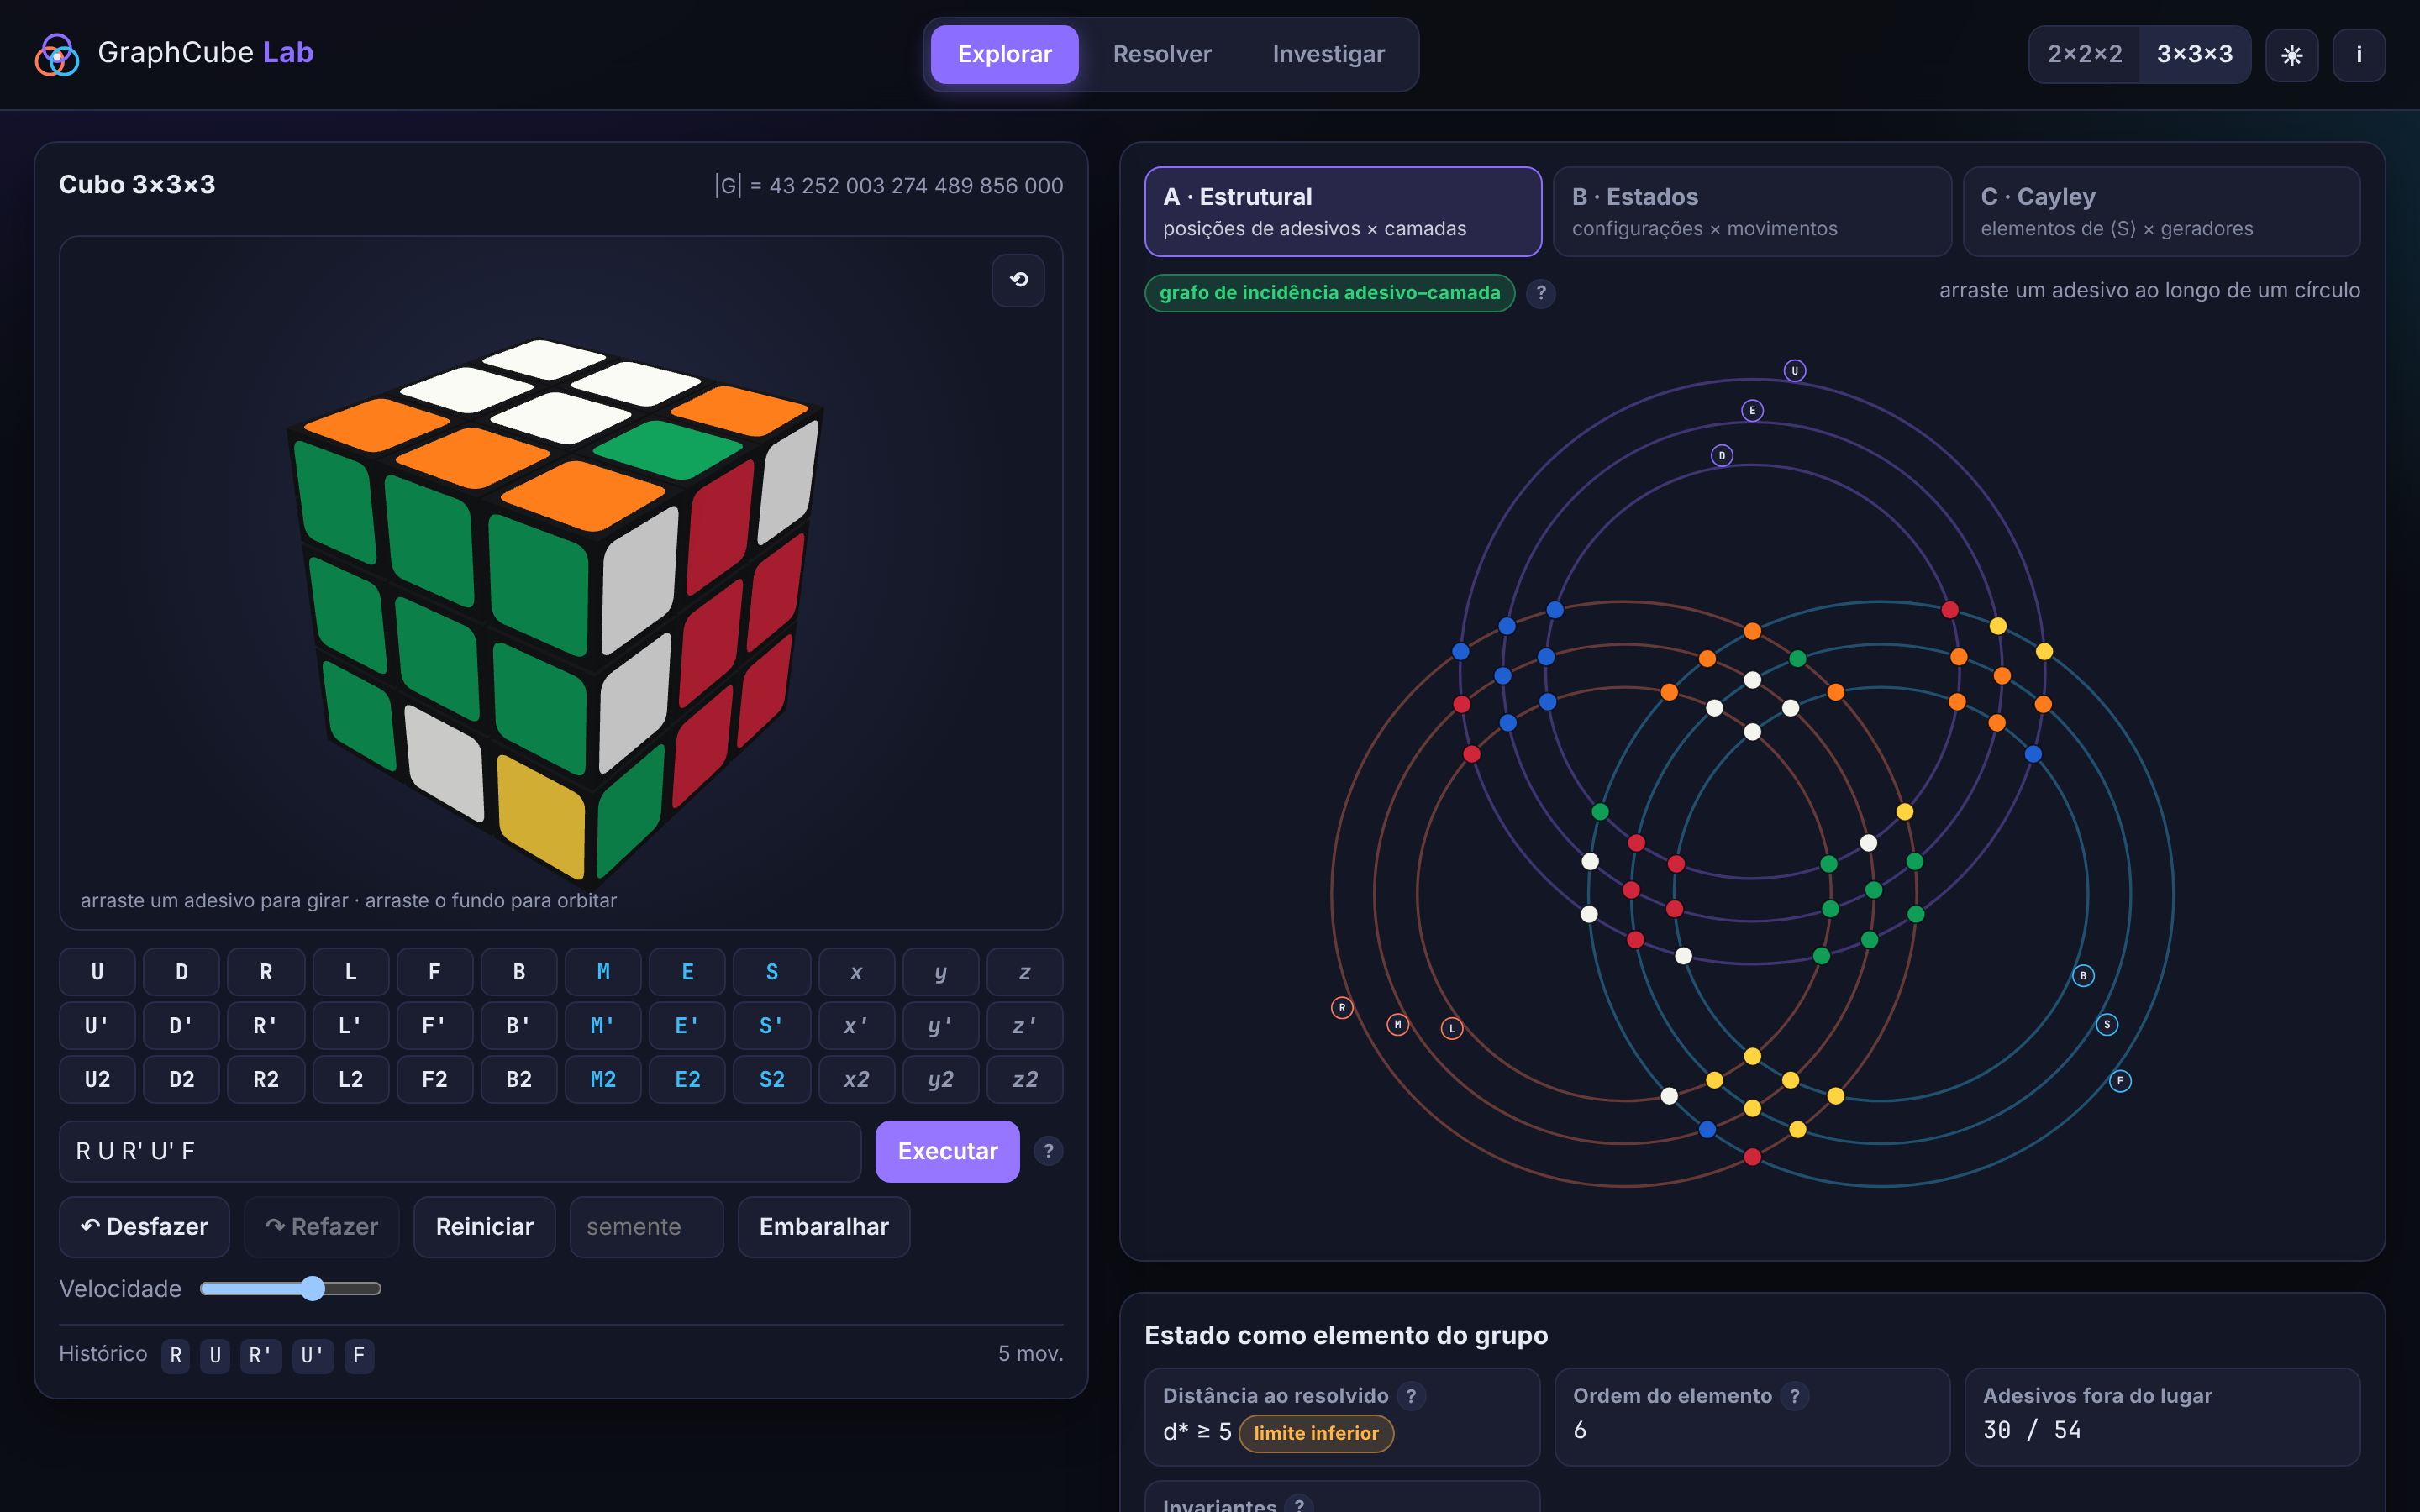
\includegraphics[width=\linewidth]{app-explorar.png}
  \caption{Modo \emph{Explorar} após \mv{R U R' U' F}: cubo 3D, grafo estrutural (posições de adesivos nas interseções dos círculos das camadas) e o estado visto como elemento do grupo (ciclos de cantos e arestas, invariantes, ordem e limite inferior para $d^*$).}
  \label{fig:interface}
\end{figure}

\begin{figure}[t]
  \centering
  \begin{subfigure}[t]{0.49\linewidth}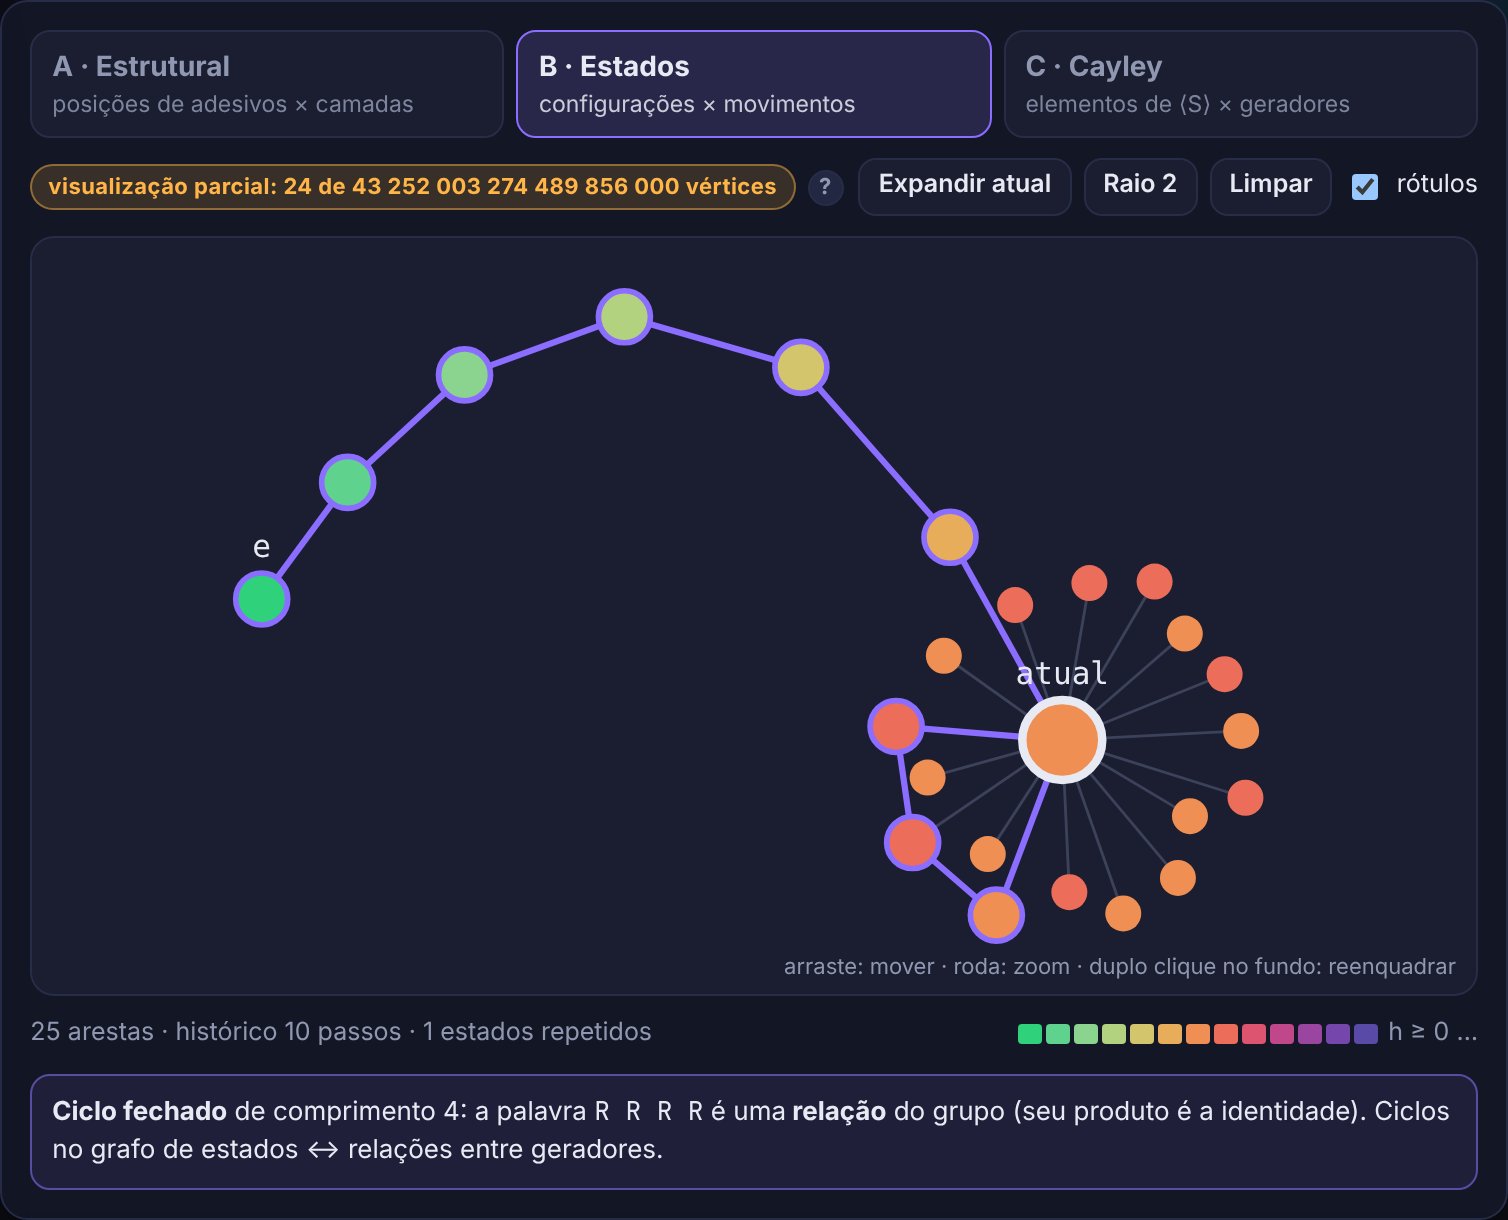
\includegraphics[width=\linewidth]{estados.png}\caption{Grafo de estados após \mv{U R R R R} e expansão local: o ciclo $\mv R^4=e$ é detectado.}\end{subfigure}\hfill
  \begin{subfigure}[t]{0.49\linewidth}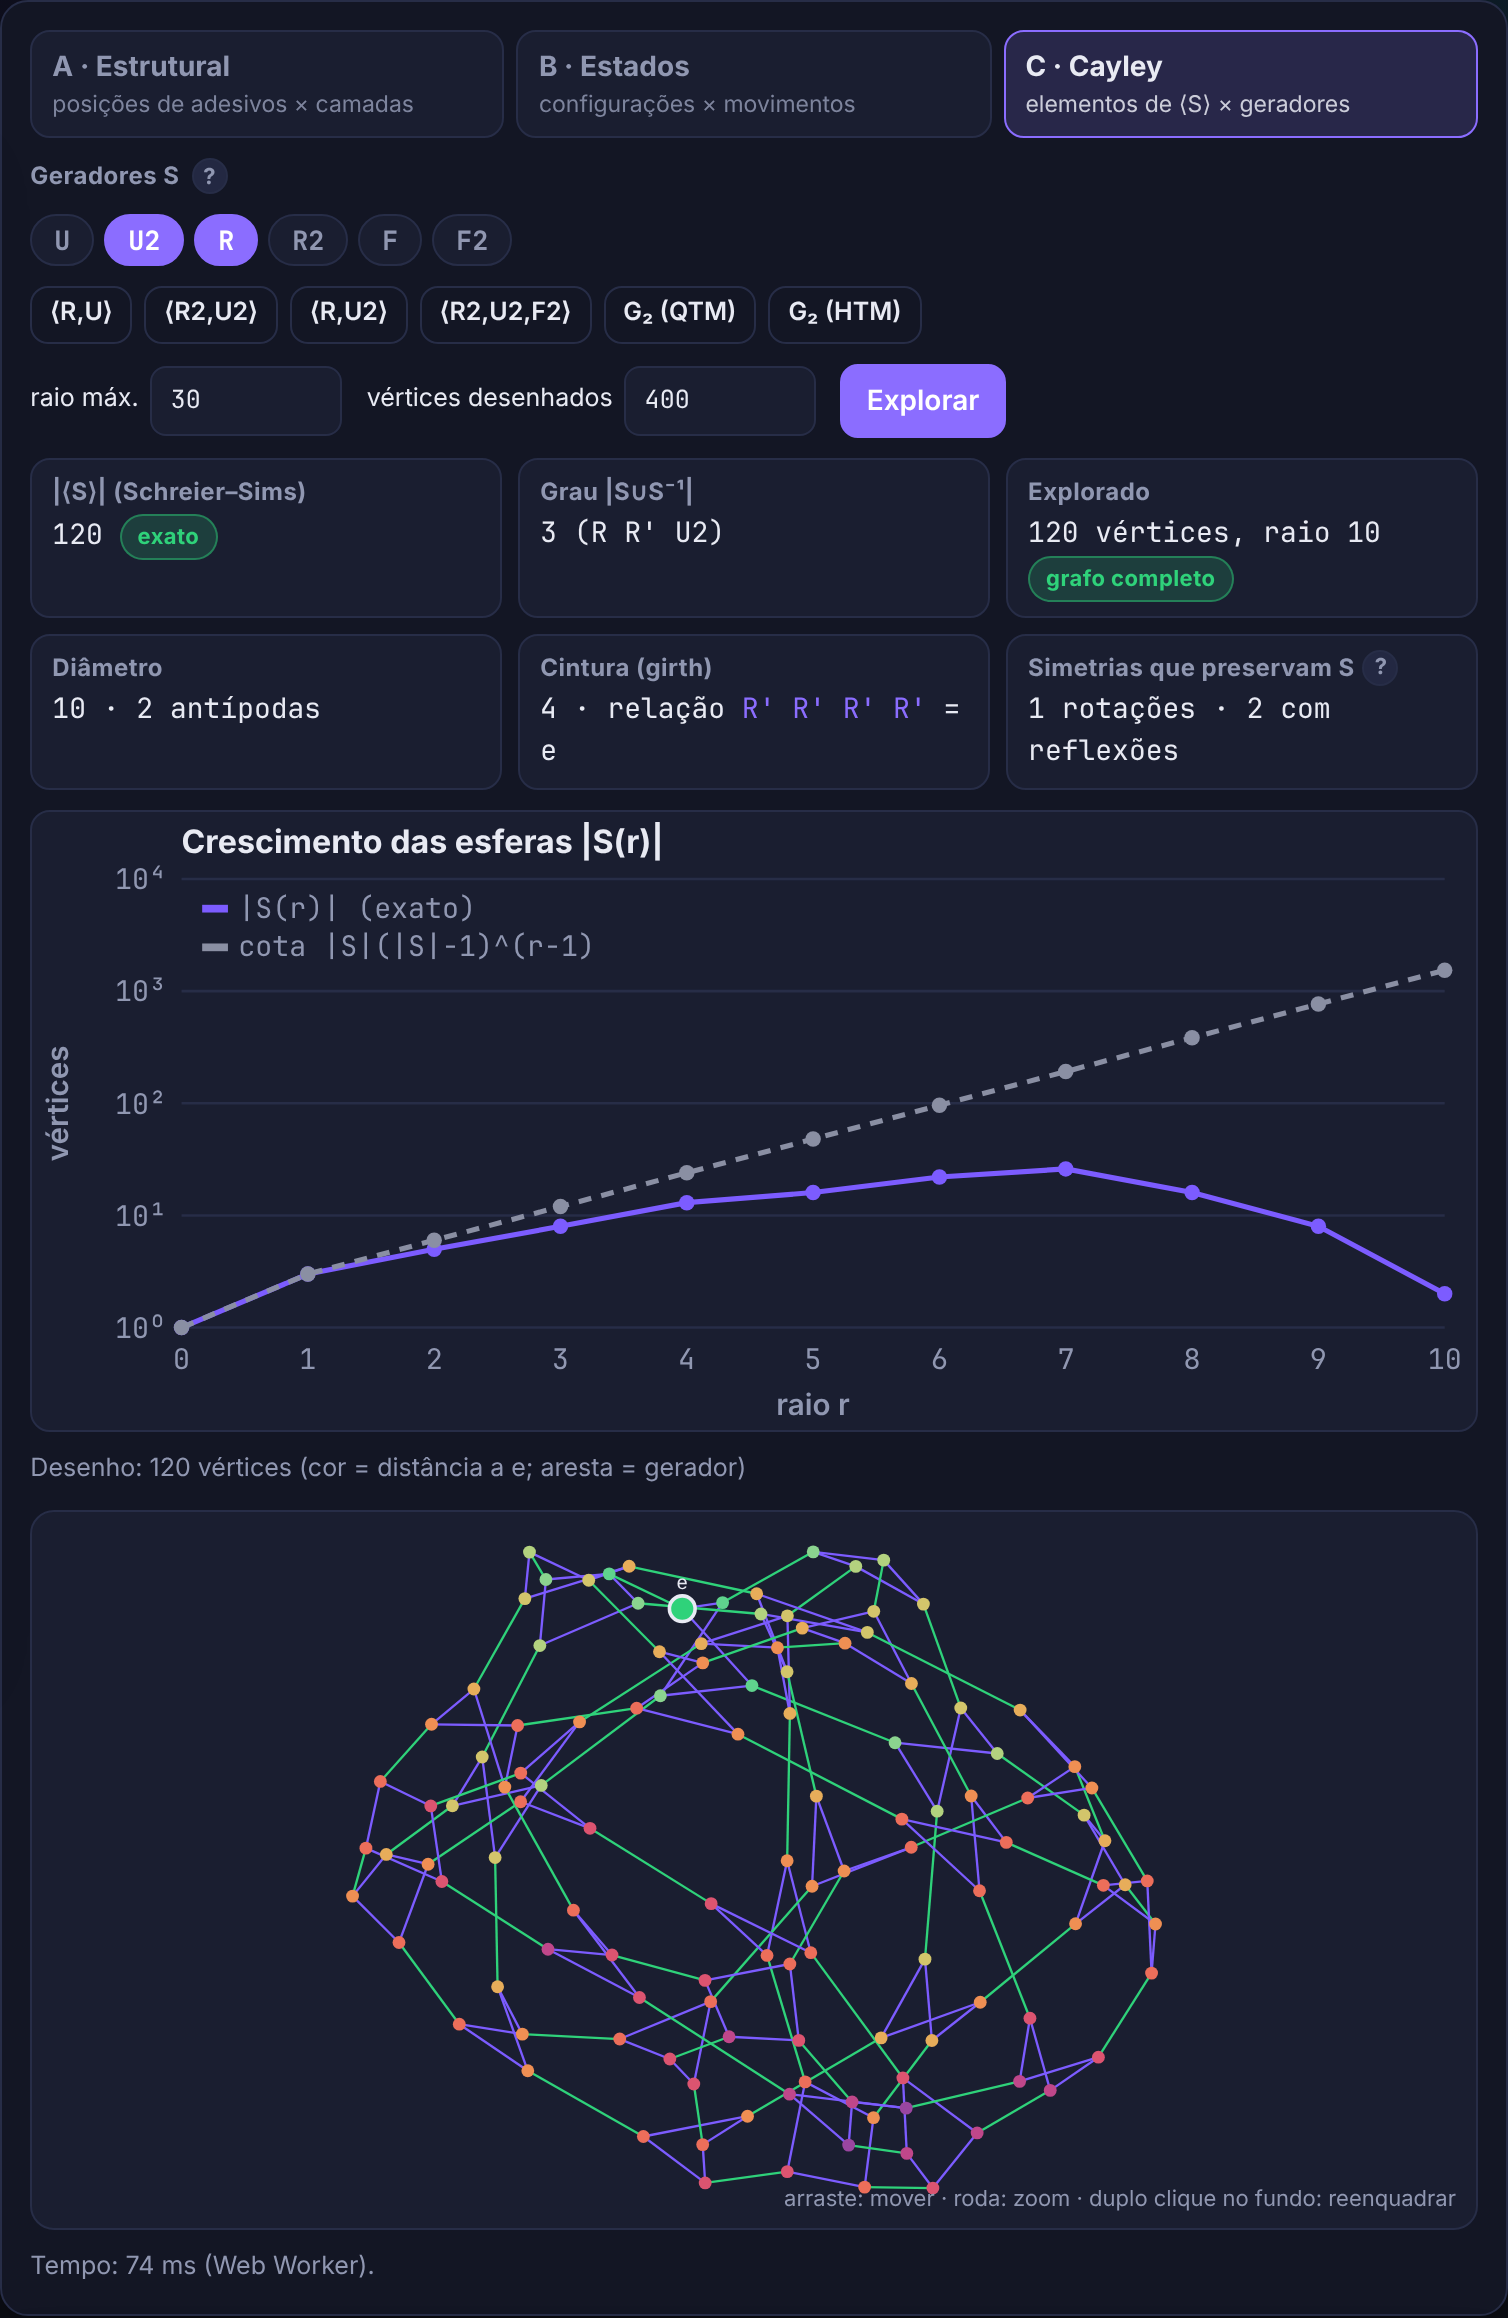
\includegraphics[width=\linewidth,trim=0 60 0 1480,clip]{cayley.png}\caption{$\Cay(\langle\mv R,\mv{U2}\rangle)$ no \cube{2}: grupo de ordem 120, diâmetro 10, cintura 4.}\end{subfigure}
  \caption{Representações (B) e (C) na interface. Os rótulos indicam quando a visualização é parcial.}
  \label{fig:grafos}
\end{figure}

\subsection{Testes}
A suíte automatizada (Vitest) tem 55 testes, organizados em: axiomas de grupo em permutações aleatórias; geometria (54 adesivos, tabelas de Kociemba, cadeias de facelets conhecidas para \mv U, \mv R, \mv F); identidade, inversos, composição e homomorfismo de palavras; ordens clássicas; comutadores, conjugados e relações entre fatias e rotações; bijeção e homomorfismo adesivos$\leftrightarrow$cubinhos; invariantes de legalidade; simetrias e referencial canônico; ordens de grupos por Schreier--Sims; distribuição de distâncias do \cube{2}; admissibilidade e consistência de todas as heurísticas em amostras; otimalidade de BFS, bidirecional, A$^*$ e IDA$^*$ contra a tabela exata; fidelidade do registro de eventos; coordenadas e tabelas de Kociemba; validade das soluções de duas fases; geometria do diagrama estrutural; propriedades de grafos de Cayley; e detecção de ciclos no grafo de estados.

\section{Metodologia experimental}\label{sec:metodologia}

\subsection{Questões e hipóteses}
\begin{description}[nosep,leftmargin=1.2em]
\item[Q1 (crescimento).] Como o esforço de busca varia com a dificuldade do problema? \emph{Hipótese:} o esforço é função da distância real $d^*$, não do comprimento $L$ do embaralhamento; $d^*$ deixa de acompanhar $L$ a partir de poucos movimentos e satura em torno da distância média do grafo.
\item[Q2 (algoritmos).] Qual o custo relativo de BFS, BFS bidirecional, A$^*$ e IDA$^*$? \emph{Hipótese:} a taxa de crescimento por camada da busca bidirecional é próxima da raiz quadrada da taxa da BFS; A$^*$/IDA$^*$ com PDBs expandem ordens de grandeza menos nós; IDA$^*$ troca memória por reexpansões.
\item[Q3 (heurísticas).] Quanto heurísticas mais informativas reduzem a busca? \emph{Hipótese:} a ordem de eficiência segue a razão média $h(s_0)/d^*$, e o máximo de duas PDBs domina cada uma delas.
\item[Q4 (estrutura).] Como o conjunto de geradores altera a estrutura de $\Cay(\langle S\rangle,S)$?
\end{description}

\subsection{Instâncias e amostragem}
\paragraph{Comprimento $L$, profundidade e distância $d^*$.} Distinguimos três grandezas que não devem ser confundidas: o \emph{comprimento do embaralhamento} $L$ (parâmetro do procedimento que gera a instância), a \emph{profundidade} atingida por uma busca (dependente do algoritmo) e a \emph{distância mínima real} $d^*(s)$ (propriedade do estado). No \cube{2}, $d^*$ é conhecido exatamente para todo estado pela tabela de 3\,674\,160 entradas; no \cube{3}, $d^*$ só é conhecido quando um algoritmo ótimo (IDA$^*$) termina.

\paragraph{Embaralhamentos.} Palavras aleatórias de comprimento $L$ sem giros consecutivos da mesma face e com faces opostas em ordem canônica (geradas por \texttt{mulberry32} com semente registrada).

\paragraph{Amostragem uniforme por camada (\cube{2}).} Para estudar os algoritmos em função de $d^*$, sorteamos índices uniformes em $[0,\num{3674160})$ e aceitamos os que têm $d^*=d$. Como a codificação é bijetiva, obtemos amostras uniformes de cada esfera $S(d)$.

\paragraph{Estados uniformes do \cube{3}.} Sorteamos independentemente $\sigma,\tau,x,y$, corrigimos a paridade trocando duas arestas e fixamos as últimas orientações pelas somas; pelo \cref{thm:lei}, isso gera estados uniformes de $G$.

\subsection{Experimentos}
\begin{description}[nosep,leftmargin=1.2em]
\item[E0 --- validação.] Ordens de sete grupos por Schreier--Sims e distribuição completa de distâncias do \cube{2} em HTM e QTM, comparadas a valores publicados.
\item[E1 --- crescimento (Q1).] \cube{2}, HTM, $L=0,\dots,\gclEoneMaxL$, \gclEoneSamples{} embaralhamentos por $L$; BFS e BFS bidirecional; registramos $d^*$ e o esforço.
\item[E2 --- algoritmos (Q2).] \cube{2}, HTM, \gclEtwoSamples{} estados uniformes em cada esfera $d^*=1,\dots,11$; BFS, bidirecional, A$^*$ e IDA$^*$ (ambos com $h_{\max}$).
\item[E3 --- heurísticas (Q3).] \cube{2}, HTM, \gclEthreeSamples{} estados uniformes em cada $d^*\in\{2,4,6,7,\allowbreak 8,9,10,11\}$; A$^*$ e IDA$^*$ com $h_0$, $h_{\mathrm{pec}}$, $h_{\mathrm{ori}}$, $h_{\mathrm{perm}}$, $h_{\max}$ e o oráculo $h^*=d^*$ (referência inferior de esforço).
\item[E3b --- \cube{3}.] \gclEthreebSamples{} embaralhamentos por $L\in\{2,4,6,7,\dots,12\}$: IDA$^*$ com $h_{\mathrm{PDB}}$ (e com $h_{\mathrm{pec}}$ para $L\le7$) e duas fases (200~ms); \gclTPUniformN{} estados uniformes de $G$ resolvidos por duas fases em dois regimes: primeira solução e ``alvo $\le20$ ou 1~s''.
\item[E4 --- estrutura (Q4).] \gclEfourSets{} conjuntos de geradores (\cref{tab:e4}); BFS a partir de $e$ (completa no \cube{2}; no \cube{3}, até \gclEfourMaxNodes{} vértices, reportando apenas esferas completas), cintura, relação mínima, simetrias e $|\langle S\rangle|$ por Schreier--Sims.
\end{description}

\subsection{Métricas e convenções}
Métrica de contagem: HTM (meia-volta conta 1), salvo indicação. Registramos: sucesso e motivo de falha (limite de nós ou de tempo); comprimento da solução e se é igual a $d^*$; nós expandidos, gerados e descobertos; pico de estados armazenados (proxy de memória --- no \cube{2} BFS e bidirecional usam tabelas de tamanho fixo de cerca de 22~MB, de modo que o pico mede o que uma implementação com tabela de dispersão precisaria guardar); tempo de parede; fator de ramificação efetivo. Execuções que estouram limites são \emph{mantidas} como falhas, não descartadas. Limites: E1/E2 $4\cdot10^6$ nós e 60~s; E3 \gclEthreeNodeLimit{} nós e 30~s; E3b $3\cdot10^7$ nós e 120~s.

\paragraph{Natureza das medidas.} São \emph{propriedades do grafo matemático} (exatas): ordens de grupos, esferas completas, diâmetros, distribuições de distâncias, cinturas e $d^*$ no \cube{2}. Dependem do \emph{procedimento de amostragem}: médias de $d^*$ em função de $L$ e qualquer média sobre instâncias. Dependem da \emph{implementação e do hardware}: tempos e contagens de nós (estas também do algoritmo e das regras de poda). Bolas desenhadas na interface são \emph{visualizações parciais}.

\subsection{Reprodutibilidade}
Cada arquivo de resultado registra experimento, parâmetros, semente efetiva, convenção de contagem, limites, versão do software, commit e ambiente. Os resultados deste artigo foram obtidos com o commit \texttt{\gclResultsCommit}, em \gclResultsEnv, em \gclResultsDate{}, num total de \gclResultsTotalMin{} minutos. Para reproduzir: \texttt{npm run experiments} (em \texttt{app/}) e \texttt{python3 experiments/analysis/analyze.py}, que regenera todas as figuras, tabelas e os números citados no texto (definidos como macros \LaTeX{} geradas a partir dos dados).

\section{Resultados}\label{sec:resultados}

Todos os valores desta seção foram produzidos pelo software descrito, com os parâmetros da \cref{sec:metodologia}; números citados no texto são gerados a partir dos arquivos de resultado.

\subsection{Validação (E0)}\label{sec:res-validacao}
A \cref{tab:e0} compara as ordens calculadas por Schreier--Sims com os valores da literatura: \gclEzeroAllMatch{} as verificações conferem\ver. A cadeia de estabilizadores de $G$ é obtida em \gclSchreierGTime~ms. A BFS completa do \cube{2} reproduz exatamente a distribuição de distâncias publicada~\cite{oeisA079761,oeisA079762,scherphuis2x2} (\cref{fig:e0}): diâmetro \gclDiamHTM{} em HTM e \gclDiamQTM{} em QTM, com distância média \gclMeanDistHTM{} (HTM) e \gclMeanDistQTM{} (QTM)\ver. As esferas iniciais de $\Cay(G,S)$ no \cube{3} calculadas no E4 também coincidem com as sequências conhecidas~\cite{oeisA080601,oeisA080583}: HTM \gclGhtmSpheres; QTM \gclGqtmSpheres\ver.

\begin{table}[t]
\centering\small
\caption{E0: ordens de grupos calculadas por Schreier--Sims e valores da literatura~\cite{joyner2008,kociembaweb,scherphuis2x2}.}\label{tab:e0}
\begin{tabular}{@{}lrrcr@{}}
\toprule
Grupo & Calculado & Literatura & Confere & ms \\
\midrule
\inputtab{generated/tables/tab_e0_groups.tex}
\bottomrule
\end{tabular}
\end{table}

\begin{figure}[t]
  \centering
  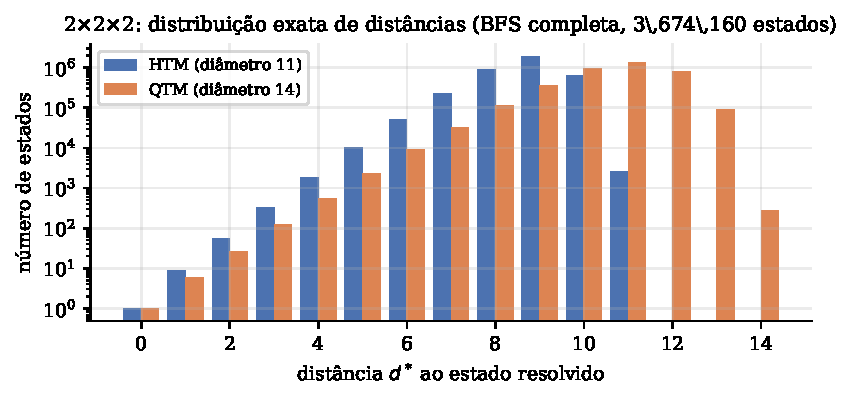
\includegraphics[width=0.86\linewidth]{fig_e0_distribution.pdf}
  \caption{E0: distribuição exata das distâncias no \cube{2} (BFS completa).}
  \label{fig:e0}
\end{figure}

\subsection{Crescimento do espaço de busca (E1)}
A \cref{fig:e1}(a) mostra que $d^*=L$ apenas para embaralhamentos muito curtos: o primeiro caso de $d^*<L$ ocorre em $L=\gclEoneFirstGap$, e para $L\ge14$ a média de $d^*$ é \gclEoneSatMean{}, praticamente a distância média uniforme \gclMeanDistHTM{}. Ou seja, $L$ é um parâmetro do procedimento, não uma medida de dificuldade. Coerentemente, a correlação de postos de Spearman entre esforço da BFS e $d^*$ é \gclEoneRhoD{}, contra \gclEoneRhoL{} com $L$. Em função de $d^*$ (\cref{fig:e1}(b)), o número médio de nós expandidos cresce geometricamente; um ajuste exponencial para $3\le d^*\le9$ dá razão por camada \gclEoneGrowthBFS{} para a BFS e \gclEoneGrowthBi{} para a BFS bidirecional, próximo de $\sqrt{\gclEoneGrowthBFS}\approx\gclEoneGrowthRatio$\proj.

\begin{figure}[t]
  \centering
  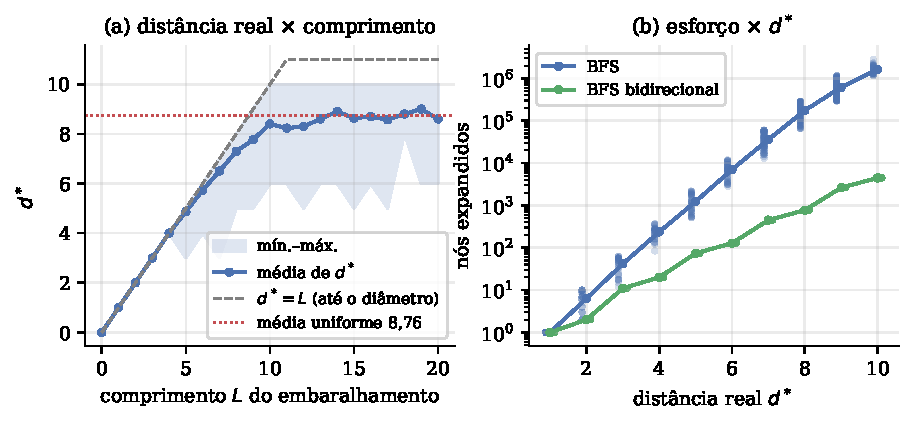
\includegraphics[width=\linewidth]{fig_e1_growth.pdf}
  \caption{E1: (a) distância real $d^*$ versus comprimento do embaralhamento; (b) nós expandidos por instância (pontos) e médias (linhas) em função de $d^*$, escala logarítmica.}
  \label{fig:e1}
\end{figure}

\subsection{Comparação de algoritmos (E2)}
Todas as \gclEtwoRuns{} execuções terminaram com sucesso dentro dos limites e \gclEtwoAllOptimal{} as soluções têm comprimento igual a $d^*$, como garantido pela teoria. A \cref{fig:e2} e a \cref{tab:e2} mostram as diferenças de custo. No caso mais difícil ($d^*=\gclEtwoDmax$), a BFS expande em média \gclEtwoBFSExp{} nós e armazena \gclEtwoBFSPeak{} estados --- praticamente todo o grupo ---, enquanto a BFS bidirecional expande \gclEtwoBFSBiExp{}. A$^*$ com $h_{\max}$ expande \gclEtwoAstarExp{} nós mas armazena \gclEtwoAstarPeak{}; IDA$^*$ expande \gclEtwoIDAstarExp{} nós (mais que A$^*$, por reexpandir nós em iterações sucessivas e não detectar repetidos), armazenando apenas o caminho corrente (\gclEtwoIDAstarPeak{} estados) e sendo o mais rápido (\gclEtwoIDAstarTime~ms de mediana).

\begin{figure}[t]
  \centering
  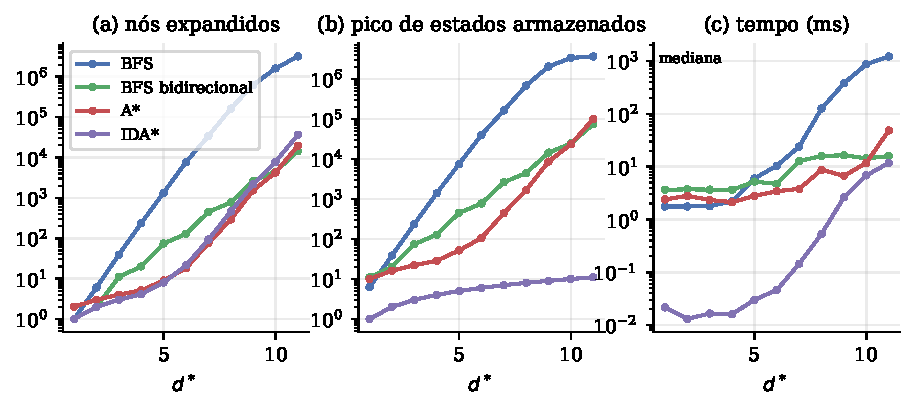
\includegraphics[width=\linewidth]{fig_e2_algorithms.pdf}
  \caption{E2: custo dos algoritmos ótimos em função de $d^*$ (\cube{2}, HTM, \gclEtwoSamples{} estados uniformes por camada).}
  \label{fig:e2}
\end{figure}

\begin{table}[t]
\centering\small
\caption{E2: resumo por algoritmo. Sucesso e otimalidade sobre todas as camadas; expandidos, pico armazenado e tempo (mediana, ms) para $d^*=\gclEtwoDmax$.}\label{tab:e2}
\begin{tabular}{@{}lrrrrr@{}}
\toprule
Algoritmo & Sucesso & Ótimas & Expandidos & Pico armaz. & Tempo \\
\midrule
\inputtab{generated/tables/tab_e2_summary.tex}
\bottomrule
\end{tabular}
\end{table}

\subsection{Heurísticas (E3)}
A \cref{tab:e3} e a \cref{fig:e3} mostram o efeito da heurística. Todas as soluções encontradas são ótimas (\gclEthreeAllOptimal), como esperado de heurísticas admissíveis. A ordem de eficiência acompanha a razão média $h(s_0)/d^*$: $h_0$ (0), $h_{\mathrm{pec}}$ (que nunca excede \gclEthreeMisMax{} no \cube{2}), $h_{\mathrm{ori}}$, $h_{\mathrm{perm}}$, $h_{\max}$ e o oráculo. Em $d^*=\gclEthreeLastD$, IDA$^*$ com $h_{\max}$ expande em média \gclEthreeMaxExp{} nós, \gclEthreeMaxOverPerm{} vezes menos que com $h_{\mathrm{perm}}$ e \gclEthreeMaxOverOri{} vezes menos que com $h_{\mathrm{ori}}$\proj. Com $h_0$, as execuções passam a estourar o limite de \gclEthreeNodeLimit{} nós a partir de $d^*=\gclEthreeZeroFailFrom$; com $h_{\mathrm{pec}}$, a partir de $d^*=\gclEthreeMisFailFrom$. Essas falhas são consequência dos limites declarados, e não de incorreção dos algoritmos. Com o oráculo, IDA$^*$ expande exatamente $d^*$ nós, o mínimo possível.

\begin{table}[t]
\centering\small
\caption{E3: média de nós expandidos por IDA$^*$ (\cube{2}, HTM, \gclEthreeSamples{} estados por camada), fator de ramificação efetivo $b^*$ em $d^*=\gclEthreeLastD$ e razão média $h(s_0)/d^*$. ``---'': todas as execuções atingiram o limite de nós; $^\dagger$: média apenas das execuções bem-sucedidas (algumas atingiram o limite).}\label{tab:e3}
\begin{tabular}{@{}l*{\gclEthreeShowCols}{r}rr@{}}
\toprule
Heurística & \inputtab{generated/tables/tab_e3_heuristics_head.tex} & $b^*$ & $h(s_0)/d^*$ \\
\midrule
\inputtab{generated/tables/tab_e3_heuristics.tex}
\bottomrule
\end{tabular}
\end{table}

\begin{figure}[t]
  \centering
  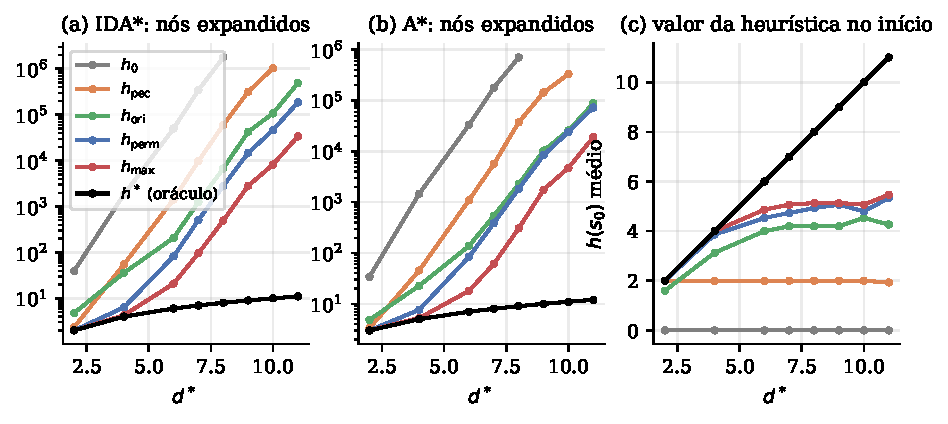
\includegraphics[width=\linewidth]{fig_e3_heuristics.pdf}
  \caption{E3: nós expandidos por IDA$^*$ (a) e A$^*$ (b) para cada heurística, e valor médio da heurística no estado inicial (c).}
  \label{fig:e3}
\end{figure}

\subsection{O \cube{3}: ótimo versus duas fases (E3b)}\label{sec:res-cube3}
Para embaralhamentos de até \gclEthreebLmax{} movimentos, IDA$^*$ com $h_{\mathrm{PDB}}$ terminou em todas as \gclEthreebCount{} instâncias, e em todas elas $d^*$ coincidiu com $L$ (\gclEthreebDstarEqLCount{} de \gclEthreebCount{}). O custo cresce rapidamente: em $L=\gclEthreebLmax$, a média foi de \gclEthreebPdbExpLast{} nós expandidos e a mediana de \gclEthreebPdbTimeLast~s (\cref{tab:e3b,fig:e3b}). A heurística $h_{\mathrm{pec}}$, executada até $L=7$, expande de 50 a 90 vezes mais nós que $h_{\mathrm{PDB}}$ em $L\in\{6,7\}$ (\cref{tab:e3b}). O método de duas fases (200~ms) encontrou a solução ótima em \gclEthreebTPOptimalPct\% das instâncias curtas, com excesso máximo de \gclEthreebTPExcessMax{} movimentos.

Em \gclTPUniformN{} estados uniformes de $G$, a \emph{primeira} solução de duas fases tem em média \gclTPFirstMean{} movimentos (de \gclTPFirstMin{} a \gclTPFirstMax; mediana de tempo \gclTPFirstTimeMed~ms); continuando a busca até obter $\le20$ ou esgotar 1~s, a média cai para \gclTPTargetMean{} (máximo \gclTPTargetMax; \gclTPTargetLe\% com $\le20$ movimentos; mediana \gclTPTargetTimeMed~ms). Nenhum desses números contradiz o diâmetro 20 de $G$~\cite{rokicki2014}: as soluções de duas fases são válidas, mas não mínimas, e o limite de tempo pode interromper a busca antes de alcançar 20.

\begin{table}[t]
\centering\small
\caption{E3b: embaralhamentos do \cube{3} (\gclEthreebSamples{} por $L$). $d^*$ é o comprimento encontrado por IDA$^*$ com $h_{\mathrm{PDB}}$ (ótimo). Tempos em ms (mediana). n.e.: não executado ($h_{\mathrm{pec}}$ apenas para $L\le7$).}\label{tab:e3b}
\begin{tabular}{@{}rrrrrrr@{}}
\toprule
& & \multicolumn{2}{c}{IDA$^*$ $h_{\mathrm{PDB}}$} & \multicolumn{2}{c}{IDA$^*$ $h_{\mathrm{pec}}$} & Duas fases \\
\cmidrule(lr){3-4}\cmidrule(lr){5-6}\cmidrule(l){7-7}
$L$ & $d^*$ & expandidos & tempo & expandidos & tempo & comprimento \\
\midrule
\inputtab{generated/tables/tab_e3b.tex}
\bottomrule
\end{tabular}
\end{table}

\begin{figure}[t]
  \centering
  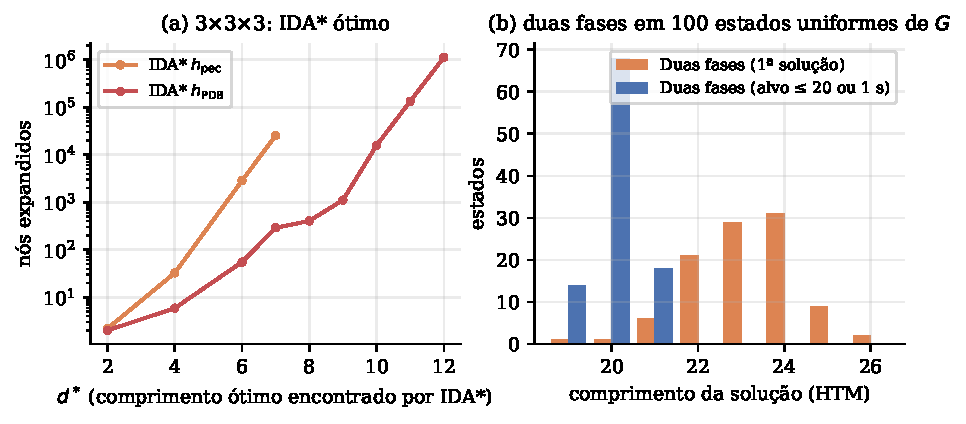
\includegraphics[width=\linewidth]{fig_e3b_cube3.pdf}
  \caption{E3b: (a) nós expandidos por IDA$^*$ no \cube{3}; (b) comprimentos das soluções de duas fases em estados uniformes de $G$.}
  \label{fig:e3b}
\end{figure}

\subsection{Estrutura dos grafos de Cayley (E4)}
A \cref{tab:e4} resume a estrutura dos \gclEfourSets{} grafos. Algumas observações\proj:
\begin{itemize}[nosep]
\item \emph{Geradores de meia-volta criam triângulos.} Incluir $X^2$ junto com $X$ produz a relação $X\,X\,X^2=e$ e cintura 3; com apenas quartos de volta, a cintura é 4 ($X^4=e$, ou um par de geradores que comutam, como $\mv{U2}\,\mv{D2}\,\mv{U2}\,\mv{D2}$ no grupo dos quadrados).
\item \emph{Grupos diédricos.} $\langle\mv{R2},\mv{U2}\rangle$ tem ordem 12 no \cube{3} (e 6 no \cube{2}): o grafo de Cayley é um ciclo de 12 vértices e a menor relação é $(\mv{U2}\,\mv{R2})^6$.
\item \emph{Mesma ordem, diâmetros diferentes.} No \cube{2}, $\langle\mv R,\mv U\rangle$ tem 29\,160 elementos e diâmetro \gclEfourRUTwoDiamQ{} em QTM, mas \gclEfourRUTwoDiamH{} quando se admitem meias-voltas. O subgrupo $\langle\mv R,\mv{U2}\rangle$ do \cube{3}, com apenas 14\,400 elementos, tem diâmetro \gclEfourRUtwoThreeDiam{}, maior que o de $G_2$: geradores ``pobres'' produzem grafos finos e longos.
\item \emph{Grupo dos quadrados.} $\langle\mv{U2},\dots,\mv{B2}\rangle$ ($663\,552$ elementos) foi enumerado completamente: diâmetro \gclEfourSqDiam{} e distância média \gclEfourSqMean{}; seu conjunto gerador é preservado pelas 48 simetrias do cubo.
\item \emph{Crescimento.} Nos grupos grandes, as esferas crescem geometricamente até a ``metade'' do grafo e depois decrescem (\cref{fig:e4}); a cota $|S|(|S|-1)^{r-1}$ só é atingida enquanto não há relações curtas.
\end{itemize}

\begin{table}[t]
\centering\footnotesize\setlength{\tabcolsep}{3.2pt}
\caption{E4: estrutura de $\Cay(\langle S\rangle,S\cup S^{-1})$. Grau $=|S\cup S^{-1}|$; ``$r\le k$'': bola exata até o raio $k$ (grafo não enumerado); diâmetro e distância média só quando completo; Sim.: simetrias do cubo (de 48) que preservam $S$.}\label{tab:e4}
\begin{tabular}{@{}lrrcrrrr@{}}
\toprule
Conjunto & $|\langle S\rangle|$ & Grau & Completo & Diâm. & Dist. média & Cintura & Sim. \\
\midrule
\inputtab{generated/tables/tab_e4.tex}
\bottomrule
\end{tabular}
\end{table}

\begin{figure}[t]
  \centering
  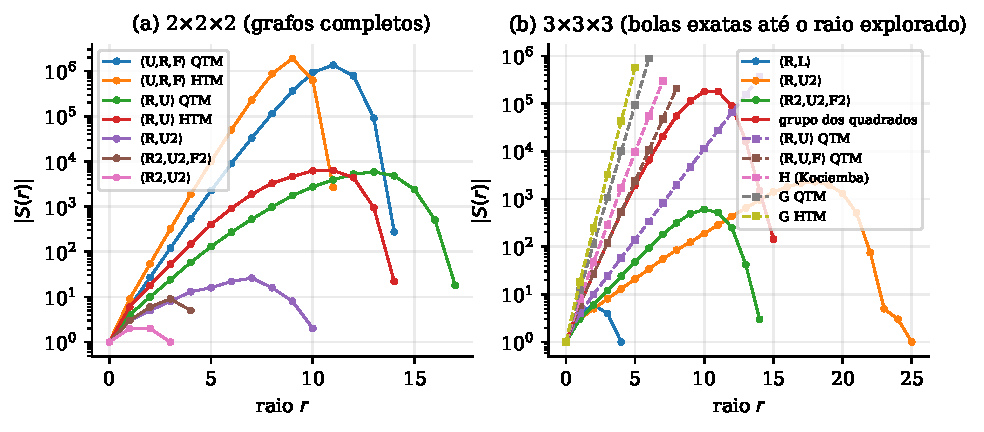
\includegraphics[width=\linewidth]{fig_e4_spheres.pdf}
  \caption{E4: tamanhos das esferas $|S(r)|$ (linhas cheias: grafos completos; tracejadas: bolas parciais, exatas até o raio mostrado).}
  \label{fig:e4}
\end{figure}

\section{Discussão}\label{sec:discussao}

\paragraph{Validação como requisito.} O fato de o núcleo reproduzir $|G|$, as ordens de seis subgrupos, a distribuição completa de distâncias do \cube{2} e as primeiras esferas do \cube{3} não é um resultado novo, mas é o que dá credibilidade aos demais. Esses testes exercitam simultaneamente a geometria dos adesivos, a convenção de composição, a conversão para cubinhos, as tabelas de coordenadas e os algoritmos de busca: um erro de sinal numa rotação, por exemplo, alteraria a distribuição de distâncias. Derivar tudo de uma única definição geométrica (em vez de tabelas digitadas) reduziu o número de pontos em que tal erro poderia ocorrer.

\paragraph{Dificuldade não é comprimento de embaralhamento.} O E1 mostra que a distância real satura muito antes do comprimento do embaralhamento e se concentra em torno da média do grafo: no \cube{2}, 75\% dos estados estão a distância 8 ou 9 (\cref{fig:e0}), e embaralhamentos de 14 ou mais movimentos já têm $d^*$ médio praticamente igual à média uniforme. Experimentos que reportam desempenho ``por número de movimentos de embaralhamento'' medem, portanto, uma mistura de dificuldades. Para o \cube{2}, em que $d^*$ é conhecido, estratificar por $d^*$ e amostrar uniformemente cada esfera (E2, E3) elimina esse viés. No \cube{3}, em que $d^*$ é desconhecido em geral, a coincidência $d^*=L$ observada para $L\le12$ é uma propriedade das instâncias geradas (embaralhamentos curtos raramente admitem atalhos), não uma lei: ela não se sustenta para $L$ próximo do diâmetro 20~\cite{rokicki2014}.

\paragraph{Algoritmos.} A razão de crescimento da BFS (\gclEoneGrowthBFS) é próxima da razão entre esferas consecutivas do \cube{2} na região intermediária ($|S(6)|/|S(5)|\approx5{,}0$), e a busca bidirecional cresce aproximadamente com a sua raiz quadrada, como prevê a análise clássica~\cite{pohl1971,russell2021}. A$^*$ e IDA$^*$ ilustram o compromisso tempo--memória: IDA$^*$ expande mais nós (reexpansões entre iterações e ausência de detecção de repetidos), mas armazena apenas o caminho e, por ter custo por nó muito menor (sem tabela de dispersão nem heap), é o mais rápido neste problema --- o mesmo motivo pelo qual Korf~\cite{korf1997} o escolheu para o \cube{3}. Tempos absolutos, contudo, dependem da implementação e do hardware e devem ser lidos apenas comparativamente.

\paragraph{Heurísticas.} A eficiência acompanha a informatividade média $h(s_0)/d^*$, e o máximo de duas PDBs pequenas (729 e 5040 entradas) supera claramente cada uma delas, como esperado: as duas projeções capturam aspectos independentes do estado (orientação e permutação). O fator de ramificação efetivo de IDA$^*$ com $h_{\max}$ ($\approx2{,}9$ em $d^*=11$) contra $\approx3{,}4$--$3{,}8$ das PDBs isoladas resume esse ganho. A heurística de contagem de peças, embora correta, é quase inútil no \cube{2} (limitada a 2) --- um exemplo de que admissibilidade não implica utilidade. A heurística aditiva~\cite{felner2004} e PDBs maiores (por exemplo, a de todos os cantos do \cube{3}, com $8!\cdot3^7\approx8{,}8\cdot10^7$ entradas~\cite{korf1997}) são extensões naturais.

\paragraph{Ótimo versus válido.} No \cube{3}, o IDA$^*$ com nossas PDBs (cerca de 2 milhões de entradas) resolve otimamente instâncias de até 12 movimentos em segundos, mas o custo cresce cerca de uma ordem de grandeza a cada movimento adicional; estados aleatórios (tipicamente a 17--18 movimentos~\cite{rokicki2014}) estão fora de alcance com essa heurística. O método de duas fases, ao contrário, resolve qualquer estado em milissegundos com soluções em torno de 20 movimentos, mas sem garantia de mínimo --- distinção que a interface torna explícita. O fato de as soluções de duas fases terem encontrado o ótimo na maioria dos embaralhamentos curtos não altera essa natureza.

\paragraph{Estrutura e geradores.} O E4 ilustra como propriedades métricas de um grafo de Cayley dependem do conjunto gerador, e não apenas do grupo: o mesmo grupo de 29\,160 elementos tem diâmetro 17 ou 14 conforme se admitam meias-voltas, e geradores ``pobres'' como $\{\mv R,\mv{U2}\}$ produzem grafos longos (diâmetro 25 com 14\,400 vértices). As relações mínimas encontradas automaticamente ($X^4$, $XXX^2$, comutação de faces opostas, $(\mv{U2}\,\mv{R2})^6$) são exatamente as relações ``óbvias'' do cubo; relações mais longas e interessantes, como $(\mv{R U R' U'})^6=e$, aparecem como ciclos mais longos que o usuário pode fechar no grafo de estados.

\paragraph{Limitações.}
(i) A análise do GraphCube baseou-se no código-fonte; a aplicação publicada e a discussão no fórum não puderam ser acessadas no ambiente de desenvolvimento.
(ii) As buscas ótimas no \cube{3} usam PDBs modestas; não reproduzimos o desempenho de Korf nem os resultados de Rokicki et al.
(iii) A memória é medida pelo número de estados armazenados, não por bytes; no \cube{2} as tabelas de acesso direto têm tamanho fixo.
(iv) Os tempos foram medidos num único ambiente virtualizado e sem repetições independentes por instância; as comparações de tempo são indicativas.
(v) A suficiência da Primeira Lei foi verificada por amostragem, não demonstrada computacionalmente; a demonstração é a da literatura~\cite{joyner2008}.
(vi) A interface foi avaliada apenas pelos autores; não houve estudo com usuários.

\section{Conclusões}\label{sec:conclusoes}

Apresentamos o GraphCube Lab, uma plataforma que parte de uma visualização existente --- o diagrama de círculos do GraphCube --- e a insere num arcabouço matemático e computacional verificável. Mostramos que o diagrama original é um grafo de incidência entre posições de adesivos e camadas, distinguimos formalmente essa estrutura do grafo de estados e dos grafos de Cayley, e implementamos as três representações de modo que cada elemento visual tenha interpretação precisa. O núcleo matemático, derivado de uma única descrição geométrica e de uma convenção de composição explícita, reproduz resultados conhecidos (ordens de grupos por Schreier--Sims e a distribuição de distâncias do \cube{2}). Os algoritmos de busca são instrumentados e visualizados a partir de seus registros reais de execução, e os experimentos são reprodutíveis a partir de sementes, metadados e um único comando.

Os experimentos quantificaram fenômenos esperados pela teoria com dados próprios: a saturação da distância real em função do comprimento do embaralhamento, a redução do crescimento por camada da busca bidirecional para aproximadamente a raiz quadrada, o ganho de combinar \textit{pattern databases} pelo máximo, o compromisso tempo--memória entre A$^*$ e IDA$^*$, o contraste entre a solução ótima viável apenas para estados próximos no \cube{3} e as soluções válidas do método de duas fases, e o efeito do conjunto gerador sobre diâmetro, cintura e simetrias de grafos de Cayley.

\paragraph{Trabalhos futuros.} (i) PDBs maiores e aditivas~\cite{korf1997,felner2004}, e redução por simetria~\cite{rokicki2014}, para ampliar o alcance das buscas ótimas no \cube{3}; (ii) cubos $n\times n\times n$ maiores, cuja geometria já é genérica no núcleo; (iii) grafos de Schreier (quocientes por subgrupos) completos e visualizáveis, como o das orientações do \cube{2}; (iv) estimativas de mistura de passeios aleatórios em grafos de Cayley; (v) avaliação da interface com estudantes, como ferramenta didática de teoria dos grupos.

\paragraph{Disponibilidade.} Código-fonte (licença MIT), dados brutos, scripts de análise e o código \LaTeX{} deste artigo estão no repositório do projeto, com instruções de reprodução no \texttt{README}.


\printbibliography[heading=bibintoc,title={Referências}]

\end{document}
